\documentclass[11pt,oneside]{article}

\usepackage[T1]{fontenc}
\usepackage[utf8]{inputenc}
\usepackage{lmodern}
\usepackage{microtype}
\usepackage[a4paper,margin=25mm,headheight=15pt]{geometry}
\usepackage{amsmath,amssymb,amsthm,mathtools,bm,mathrsfs}
\usepackage{booktabs,longtable,tabularx,array,multirow}
\usepackage{graphicx}
\usepackage{caption}
\usepackage{float}
\usepackage{enumitem}
\usepackage{xcolor}
\usepackage{xurl}
\usepackage{hyperref}
\usepackage[nameinlink,capitalise,noabbrev]{cleveref}
\usepackage{fancyhdr}
\usepackage{listings}
\usepackage{setspace}

\definecolor{navy}{HTML}{17365D}
\definecolor{teal}{HTML}{176B67}
\definecolor{burgundy}{HTML}{7A2848}
\definecolor{gold}{HTML}{A27117}
\definecolor{slate}{HTML}{4B5968}
\definecolor{lightblue}{HTML}{EEF4FA}
\definecolor{lightgreen}{HTML}{EEF8F4}
\definecolor{lightgold}{HTML}{FFF8E7}
\definecolor{lightred}{HTML}{FBEFF3}
\definecolor{lightgray}{HTML}{F4F6F8}

\hypersetup{
  colorlinks=true,
  linkcolor=navy,
  citecolor=teal,
  urlcolor=burgundy,
  pdftitle={Exact Information Geometry and New Frontiers for the Fabius--Rvachev System},
  pdfauthor={OpenAI GPT-5.6 Pro},
  pdfsubject={Fabius function, Rvachev up-function, Thue--Morse sequence, q-analogs, information theory, Fisher information, Lambert W},
  pdfkeywords={Fabius, Rvachev, Thue-Morse, q-series, sinc products, Bell polynomials, Bernoulli numbers, Lambert W, entropy, Fisher information}
}

\pagestyle{fancy}
\fancyhf{}
\fancyhead[L]{\small\textsc{Fabius--Rvachev information geometry}}
\fancyhead[R]{\small\thepage}
\fancyfoot[C]{}
% Canonical project-wide mathematical notation.
% Canonical mathematical notation for active FabiusFunction LaTeX documents.
%
% This file is intentionally a plain TeX input rather than a LaTeX package.
% Every standalone document loads it by an explicit path relative to that
% document's directory; included fragments inherit the definitions from their
% root document.  Keep this file independent of document layout and metadata.
%
% Contract:
%   * one command has one mathematical meaning throughout the active corpus;
%   * names encode semantic roles rather than a document-local choice of letter;
%   * visually similar but differently normalized objects have different print;
%   * every command below is defined normatively in the notation catalogue.
%
% The active corpus excludes docs/archive/.  Historical sources may retain
% their original notation only inside an explicitly labelled quotation.

\makeatletter
\@ifundefined{mathbb}{%
  \PackageError{fabius-notation}{The amssymb package must be loaded first}%
    {Load amsmath and amssymb before inputting fabius-notation.tex.}%
}{}
\@ifundefined{operatorname}{%
  \PackageError{fabius-notation}{The amsmath package must be loaded first}%
    {Load amsmath before inputting fabius-notation.tex.}%
}{}
\makeatother

% Version stamp used by the catalogue and by static audits.
\newcommand{\FabiusNotationVersion}{2026-08-31}

% Number systems.  NaturalNumbers is explicitly the nonnegative convention.
\newcommand{\NaturalNumbers}{\mathbb{N}_{0}}
\newcommand{\PositiveIntegers}{\mathbb{N}_{>0}}
\newcommand{\IntegerNumbers}{\mathbb{Z}}
\newcommand{\RationalNumbers}{\mathbb{Q}}
\newcommand{\RealNumbers}{\mathbb{R}}
\newcommand{\ComplexNumbers}{\mathbb{C}}
\newcommand{\ExtendedRealNumbers}{\overline{\mathbb{R}}}

% The three principal Fabius--Rvachev functions.  Subscripts are deliberate:
% a bare F and a calligraphic F have several unrelated uses in the corpus.
\newcommand{\FabiusBounded}{F_{\mathrm{bd}}}
\newcommand{\FabiusGlobal}{F_{\mathrm{gl}}}
\newcommand{\FabiusQuantile}{Q_{F}}
\newcommand{\FabiusClampedQuantile}{Q_{F,\mathrm{cl}}}
\newcommand{\RvachevUp}{\operatorname{up}}

% Constants, elementary operators, and delimiters.
\newcommand{\EulerE}{\mathrm{e}}
\newcommand{\ImaginaryUnit}{\mathrm{i}}
\newcommand{\Differential}{\mathop{}\!\mathrm{d}}
\newcommand{\AbsoluteValue}[1]{\left\lvert #1\right\rvert}
\newcommand{\Norm}[1]{\left\lVert #1\right\rVert}
\newcommand{\Floor}[1]{\left\lfloor #1\right\rfloor}
\newcommand{\Ceiling}[1]{\left\lceil #1\right\rceil}
\newcommand{\FractionalPart}[1]{\left\{#1\right\}}
\newcommand{\PositivePart}[1]{\left(#1\right)_{+}}
\newcommand{\IndicatorOf}[1]{\mathbf{1}_{#1}}
\newcommand{\SetOf}[1]{\left\{#1\right\}}
\newcommand{\InnerProduct}[1]{\left\langle #1\right\rangle}
\newcommand{\CardinalityOf}[1]{\left\lvert #1\right\rvert}
\newcommand{\DefinitionEquals}{\mathrel{\coloneqq}}
\newcommand{\Sign}{\operatorname{sgn}}
\newcommand{\IdentityOperator}{\operatorname{id}}
\newcommand{\SpanOperator}{\operatorname{span}}
\newcommand{\TraceOperator}{\operatorname{tr}}
\newcommand{\RankOperator}{\operatorname{rank}}
\newcommand{\DiagonalOperator}{\operatorname{diag}}
\newcommand{\ResidueOperator}{\operatorname*{Res}}
\newcommand{\LeastCommonMultiple}{\operatorname{lcm}}
\newcommand{\OrderOperator}{\operatorname{ord}}
\newcommand{\PrincipalLogarithm}{\operatorname{Log}}
\newcommand{\FallingFactorial}[2]{\left(#1\right)^{\underline{#2}}}
\newcommand{\RisingFactorial}[2]{\left(#1\right)^{\overline{#2}}}

% Support, topology, convolution, and metric notation.
\newcommand{\SupportOperator}{\operatorname{supp}}
\newcommand{\SupportOf}[1]{\SupportOperator\!\left(#1\right)}
\newcommand{\TopologicalSupportOf}[1]{\operatorname{tsupp}\!\left(#1\right)}
\newcommand{\Convolution}{\mathbin{*}}
\newcommand{\MetricDistance}{\operatorname{dist}}
\newcommand{\TotalVariationDistance}{d_{\mathrm{TV}}}

% Probability.  Equality and convergence in law are not metric distance.
\newcommand{\Probability}{\mathbb{P}}
\newcommand{\Expectation}{\mathbb{E}}
\newcommand{\Variance}{\operatorname{Var}}
\newcommand{\Covariance}{\operatorname{Cov}}
\newcommand{\LawOperator}{\operatorname{Law}}
\newcommand{\LawOf}[1]{\LawOperator\!\left(#1\right)}
\newcommand{\EqualInLaw}{\mathrel{\overset{\mathrm{law}}{=}}}
\newcommand{\ConvergesInLaw}{\mathrel{\xrightarrow{\mathrm{law}}}}

% Fourier and integral transforms.  The printed labels expose normalization.
% FourierTwoPi uses exp(-2*pi*i*x*xi); FourierAngular uses exp(-i*x*omega).
\newcommand{\FourierTwoPi}[1]{\widehat{#1}_{\,2\pi}}
\newcommand{\FourierAngular}[1]{\widehat{#1}_{\,\mathrm{ang}}}
\newcommand{\LaplaceTransformSymbol}{\mathcal{L}}
\newcommand{\MellinTransformSymbol}{\mathcal{M}}
\newcommand{\LaplaceTransformOf}[1]{\LaplaceTransformSymbol\!\left[#1\right]}
\newcommand{\MellinTransformOf}[1]{\MellinTransformSymbol\!\left[#1\right]}
\newcommand{\MomentGeneratingFunction}[1]{M_{#1}}
\newcommand{\CharacteristicFunction}[1]{\varphi_{#1}}

% The two standard sinc functions must never share one symbol.
\newcommand{\SincRad}{\operatorname{sinc}_{\mathrm{rad}}}
\newcommand{\SincPi}{\operatorname{sinc}_{\pi}}

% Binary arithmetic and Thue--Morse notation.
\newcommand{\BinaryDigitSum}{\operatorname{wt}_{2}}
\newcommand{\ThueMorseSignSymbol}{\varepsilon}
\newcommand{\ThueMorseSign}[1]{\varepsilon_{#1}}
\newcommand{\PadicValuation}[1]{\nu_{#1}}
\newcommand{\TwoAdicValuation}{\nu_{2}}

% q-series notation.  Every base is an explicit argument.
\newcommand{\QPochhammer}[3]{\left(#1;#2\right)_{#3}}
\newcommand{\GaussianBinomial}[3]{%
  \genfrac{[}{]}{0pt}{}{#1}{#2}_{#3}%
}
\newcommand{\QInteger}[2]{\left[#1\right]_{#2}}

% Named special functions.
\newcommand{\Polylogarithm}{\operatorname{Li}}
\newcommand{\LambertW}{W}
\newcommand{\GammaFunction}{\Gamma}
\newcommand{\RiemannZeta}{\zeta}

% Asymptotics.  BigO and LittleO are operator tokens for existing formula
% grammar; prefer the At forms so that the limiting regime is printed.
\newcommand{\BigO}{\mathcal{O}}
\newcommand{\LittleO}{o}
\newcommand{\BigOAt}[2]{\mathcal{O}_{#2}\!\left(#1\right)}
\newcommand{\LittleOAt}[2]{o_{#2}\!\left(#1\right)}

\renewcommand{\headrulewidth}{0.4pt}

\setlength{\parindent}{0pt}
\setlength{\parskip}{0.55em}
\setlength{\emergencystretch}{2em}
\setlist[itemize]{leftmargin=1.8em,itemsep=0.3ex,topsep=0.4ex}
\setlist[enumerate]{leftmargin=2.1em,itemsep=0.35ex,topsep=0.45ex}
\allowdisplaybreaks
\graphicspath{{figures/}}

\newtheorem{theorem}{Theorem}[section]
\newtheorem{proposition}[theorem]{Proposition}
\newtheorem{corollary}[theorem]{Corollary}
\newtheorem{lemma}[theorem]{Lemma}
\newtheorem{conjecture}[theorem]{Conjecture}
\newtheorem{problem}[theorem]{Problem}
\theoremstyle{definition}
\newtheorem{definition}[theorem]{Definition}
\newtheorem{example}[theorem]{Example}
\newtheorem{experiment}[theorem]{Numerical experiment}
\theoremstyle{remark}
\newtheorem{remark}[theorem]{Remark}

\newcommand{\Corr}{\operatorname{Corr}}
\newcommand{\KL}{D_{\mathrm{KL}}}
\newcommand{\MI}{I}
\newcommand{\mmse}{\operatorname{mmse}}
\newcommand{\ind}{\mathbf 1}
\newcommand{\epsTM}{\varepsilon}
\newcommand{\Repo}{\textcolor{navy}{\textbf{[repository input]}}}
\newcommand{\New}{\textcolor{teal}{\textbf{[proved here]}}}
\newcommand{\Derived}{\textcolor{gold}{\textbf{[derived synthesis]}}}
\newcommand{\Numerical}{\textcolor{burgundy}{\textbf{[numerical]}}}
\newcommand{\Conj}{\textcolor{burgundy}{\textbf{[conjecture]}}}

\newenvironment{resultbox}[1][Frontier result]{%
  \par\medskip\noindent
  \begin{center}\begin{minipage}{0.94\textwidth}
  \color{black}\hrule\vspace{0.55em}
  \textbf{#1.}\quad
}{%
  \vspace{0.55em}\hrule
  \end{minipage}\end{center}\medskip
}

\lstdefinestyle{pythonstyle}{
  language=Python,
  basicstyle=\ttfamily\small,
  columns=fullflexible,
  keepspaces=true,
  showstringspaces=false,
  breaklines=true,
  frame=single,
  backgroundcolor=\color{lightgray},
  commentstyle=\itshape\color{slate},
  keywordstyle=\bfseries\color{navy},
  xleftmargin=0.4em,
  xrightmargin=0.4em
}

\title{\bfseries Exact Information Geometry and New Frontiers\\[0.35em]
\Large for the Fabius Function, Rvachev's Up-Function,\\
Thue--Morse Sinc Products, and Geometric $q$-Convolutions}
\author{Research report prepared for Vladimir Reshetnikov\\
\small Repository-aware analysis, exact proofs, and reproducible experiments}
\date{30 August 2026}

\begin{document}
\maketitle

\begin{abstract}
The Fabius--Rvachev corpus already connects the Thue--Morse sequence, exact dyadic
arithmetic, $q$-binomial interpolation, infinite sinc products, Bell--Bernoulli
moment calculus, Legendre expansions, inverse functions, and lower-Lambert
endpoint asymptotics.  This report develops a different, previously unexploited
organizing layer: the exact information carried by each geometric convolution
scale.

For
\[
 X_q=(1-q)\sum_{j\ge0}q^jU_j,
 \qquad U_j\stackrel{\mathrm{iid}}\sim\mathrm{Unif}[-1,1],
 \qquad 0<q<1,
\]
let $S_{q,m}$ be the first $m$ summands.  The self-similar tail identity
$X_q=S_{q,m}+q^mX_q'$ implies the exact non-Gaussian channel law
\[
 I(X_q;S_{q,m})=m\log(1/q),
 \qquad
 \operatorname{mmse}(X_q\mid S_{q,m})=q^{2m}\operatorname{Var}(X_q),
\]
and, strikingly,
\[
 I(X_q;S_{q,m})=-\frac12\log\!\bigl(1-\Corr(X_q,S_{q,m})^2\bigr),
\]
the familiar Gaussian correlation formula holding here for a compactly supported,
nowhere-analytic density.  Every new geometric digit contributes exactly
$\log(1/q)$ nats conditionally.  The scalar prefix is a sufficient statistic for
the entire digit block, and its posterior is an exact translated, rescaled copy of
the original Fabius--Rvachev law.  This yields closed posterior cumulants, Bell
moments, quantiles, R\'enyi entropies, Fisher information, and transported
Legendre expansions.

At $q=1/2$, the finite prefix density is a Thue--Morse signed spline.  Substitution
into the posterior formula gives an exact Kullback--Leibler integral equaling
$m\log2$, thereby joining a finite Thue--Morse product to the infinite Rvachev
sinc product in one Bayesian identity.  The centered information density converges
to a difference of two independent Rvachev surprisals; its limiting variance is
twice the varentropy and its cumulant generating function is a symmetric pair of
R\'enyi integrals.

A second main theorem identifies the first entropy correction of the finite sinc
prefixes:
\[
 h(X_q)-h(S_{q,m})
 =\frac{\operatorname{Var}(X_q)\,\mathcal J(f_q)}2q^{2m}
  +o(q^{2m}),
\]
where $\mathcal J$ is Fisher information.  In the dyadic case a new bridge gives
\[
 \mathcal J(\RvachevUp)
 =\int_0^1\frac{F'(x)^2}{F(x)(1-F(x))}\Differential x
 =\int_0^1\frac{\Differential y}{y(1-y)(F^{-1})'(y)}.
\]
Combining the inverse-Fabius elasticity with the lower-Lambert scale produces a
new endpoint entropy law.  Finally, exact Bernoulli cumulants yield a formal
entropic Edgeworth expansion as $q\uparrow1$; the report isolates the remaining
uniform-analysis step as a precise conjecture and tests it numerically.  All
claims are status-labeled, and the archive contains the complete LaTeX source,
compiled PDF, commented Python code, exact symbolic checks, CSV data, and vector
figures.
\end{abstract}

\tableofcontents
\newpage

\section{Scope, corpus audit, and contribution boundary}
\label{sec:scope}

\subsection{What was audited}

The source audit covered the recursive LaTeX corpus under
\path{Analysis/FabiusFunction/docs} in the current \texttt{ProveIt} tree, including
the primary exposition, glossary, Lean walkthrough, active semi-formalized and
non-formalized frontier volumes, archived studies, representation drafts,
inverse-and-sampling drafts, $q$-series drafts, and the recent parallel reports
mirrored in the working library.  The audit was claim-oriented rather than merely
title-oriented: theorem statements, conclusion sections, imported-interface
lists, and exact or close-variant phrase searches were checked for the proposed
notions ``mutual information'', ``MMSE'', ``rate distortion'', ``information
density'', ``varentropy'', ``finite-prefix entropy'', and ``Fisher information''.

The following are treated strictly as imported inputs and are not relabeled as
new:
\begin{itemize}
\item the random-uniform series for the Fabius/Rvachev law, its refinement and
      differential-dilation equations, and its infinite sinc product;
\item exact dyadic values, Thue--Morse derivative and truncated-power formulas,
      rational moments, and the Bell--Bernoulli cumulant calculus;
\item the geometric-$q$ family, Gaussian-binomial interpolation, reciprocal-$q$
      deconvolution, negative-$q$ affine dualities, and finite convolution models;
\item inverse-Fabius algebraic germs, inverse derivative recurrences, and the
      phase-aware all-orders lower-Lambert endpoint calculus;
\item Legendre, Jacobi, Lagrange, sampling, multiresolution, Fredholm, resolvent,
      Appell, Stein, and Koopman representations already developed in the corpus;
\item the existing global entropy identity
      $\int_0^1\log (F^{-1})'(y)\Differential y=h(F')$ and entropy laws for derivative-energy
      measures in the non-dyadic atomic-function hierarchy.
\end{itemize}

The phrase ``new'' below therefore means \emph{not located in the audited repository
corpus under the displayed normalization}.  It is not an unconditional claim of
worldwide publication priority.  Several abstract ingredients, such as Shannon's
lower bound, entropy power, high-resolution rate distortion, Fisher information,
and entropic Edgeworth expansions, have substantial external literatures.  The
frontier contribution is their exact synthesis with the geometric Fabius--Rvachev
convolution and its Thue--Morse, inverse, and Lambert structures.

\subsection{Result ledger}

\begin{longtable}{@{}p{0.34\textwidth}p{0.15\textwidth}p{0.42\textwidth}@{}}
\toprule
Result & Status & Main mechanism \\
\midrule
\endfirsthead
\toprule
Result & Status & Main mechanism \\
\midrule
\endhead
Exact prefix mutual information $I(X_q;S_{q,m})=m\log(1/q)$ & proved & independent self-similar tail \\
Constant information per geometric digit & proved & chain rule and prefix sufficiency \\
Posterior location-scale copy, quantiles, cumulants, Bell moments, R\'enyi and Fisher scaling & proved & conditional density formula \\
Non-Gaussian Gaussian-correlation identity and exact MMSE & proved & orthogonal projection onto the prefix \\
Rate-distortion bracket and asymptotic prefix-code gap & derived & Shannon lower bound and high-resolution theory \\
Finite Thue--Morse spline Bayesian/KL identity & proved & inclusion-exclusion spline plus Rvachev posterior \\
Information-spectrum limit and R\'enyi cumulant generating function & proved & independent-tail coupling \\
Finite-sinc entropy correction governed by Fisher information & proved & Fourier deconvolution and entropy variation \\
Fisher bridge through $F$, $F^{-1}$, and $\RvachevUp$ & proved & symmetry, differentiation, and quantile transport \\
Lower-Lambert endpoint tail-entropy law & derived from audited asymptotics & inverse elasticity and Watson integration \\
Entropic Edgeworth coefficients $3/100$ and $33/500$ near $q=1$ & formal plus numerical & Bernoulli cumulants and Hermite orthogonality \\
Full entropic $q\uparrow1$ expansion and monotonic deficit & conjectural & uniform Fourier/entropy control \\
\bottomrule
\end{longtable}

\begin{resultbox}[Central new principle]
The geometric convolution is not only a product representation of a density.  It
is an exact equal-information filtration: observing one additional uniform scale
always reveals precisely $\log(1/q)$ nats about the final random variable,
independently of the depth and despite the strongly non-Gaussian posterior.
\end{resultbox}

\section{The geometric-uniform family and the dyadic dictionary}
\label{sec:family}

\subsection{Probability law, fixed point, and Fourier product}

Let $U_0,U_1,\ldots$ be independent $\mathrm{Unif}[-1,1]$ random variables and set
\begin{equation}
 X_q=(1-q)\sum_{j=0}^{\infty}q^jU_j,
 \qquad 0<q<1.
 \label{eq:Xq}
\end{equation}
The series converges absolutely and $X_q\in[-1,1]$.  Write $f_q$ for its density,
$F_q$ for its distribution function, and
\begin{equation}
 \phi_q(t)=\Expectation\EulerE^{\ImaginaryUnit tX_q}
 =\prod_{j=0}^{\infty}\SincRad\bigl((1-q)q^jt\bigr),
 \qquad \SincRad z=\frac{\sin z}{z}.
 \label{eq:phi-q}
\end{equation}
The first digit gives the distributional fixed point
\begin{equation}
 X_q\stackrel d=qX_q'+(1-q)U_0,
 \label{eq:fixedpoint}
\end{equation}
where $X_q'$ is an independent copy.  Consequently
\begin{equation}
 f_q(x)=\frac{F_q((x+1-q)/q)-F_q((x-1+q)/q)}{2(1-q)}.
 \label{eq:density-transfer}
\end{equation}
The product in \eqref{eq:phi-q} decays faster than every power on the real line;
thus $f_q\in C_c^\infty(\RealNumbers)$ and is flat at the support endpoints.  These regularity
facts are repository inputs, but they are also immediate from the standard
``number of active sinc factors'' estimate.

\subsection{Variance, Bernoulli cumulants, and Bell moments}

Since $\Variance(U_j)=1/3$,
\begin{equation}
 \sigma_q^2:=\Variance(X_q)=\frac{(1-q)^2}{3}\sum_{j\ge0}q^{2j}
 =\frac{1-q}{3(1+q)}.
 \label{eq:variance}
\end{equation}
The logarithm of $\sinh z/z$ gives the even cumulants
\begin{equation}
 \kappa_{2r}(X_q)
 =\frac{2^{2r}B_{2r}}{2r}\,
   \frac{(1-q)^{2r}}{1-q^{2r}},
 \qquad
 \kappa_{2r+1}(X_q)=0.
 \label{eq:cumulants}
\end{equation}
Here $B_n$ are the Bernoulli numbers with $B_2=1/6$.  Every ordinary moment is
therefore a complete Bell polynomial:
\begin{equation}
 \mu_n(q):=\Expectation X_q^n
 =\mathcal B_n\bigl(0,\kappa_2,0,\kappa_4,\ldots,\kappa_n\bigr).
 \label{eq:Bell-moments}
\end{equation}
This imported Bell--Bernoulli interface will make the posterior moment formulas
below completely explicit.

\subsection{The Fabius--Rvachev specialization}

At $q=1/2$, write $X=X_{1/2}$.  In the probability normalization used here,
\begin{equation}
 \Probability(X\in\Differential x)=\RvachevUp(x)\Differential x,
 \qquad -1\le x\le1,
 \label{eq:up-density}
\end{equation}
and the affine variable $Y=(X+1)/2$ has the Fabius distribution:
\begin{equation}
 \Probability(Y\le y)=F(y),
 \qquad F'(y)=2\RvachevUp(2y-1),
 \qquad 0<y<1.
 \label{eq:F-density}
\end{equation}
Equivalently,
\begin{equation}
 \RvachevUp(x)=F(1-\AbsoluteValue{x}),\qquad \AbsoluteValue{x}\le1.
 \label{eq:up-F}
\end{equation}
Let
\begin{equation}
 G=F^{-1}:(0,1)\longrightarrow(0,1)
 \label{eq:G}
\end{equation}
be the inverse Fabius function.  The variance is
\begin{equation}
 \Variance(X)=\frac19.
 \label{eq:dyadic-var}
\end{equation}
The report will move repeatedly among the centered density $\RvachevUp$, the bounded CDF
$F$, and the quantile $G$; \eqref{eq:F-density} fixes every factor of two.

\section{An exact equal-information filtration}
\label{sec:exact-info}

\subsection{Prefix and tail decomposition}

For $m\ge1$, define the finite geometric prefix
\begin{equation}
 S_{q,m}=(1-q)\sum_{j=0}^{m-1}q^jU_j.
 \label{eq:prefix}
\end{equation}
Let $X_q^{(m)}$ be an independent copy of $X_q$, formed from the tail digits.  Then
\begin{equation}
 X_q=S_{q,m}+q^mX_q^{(m)},
 \qquad S_{q,m}\perp X_q^{(m)}.
 \label{eq:tail-decomposition}
\end{equation}
This elementary identity is the engine behind all exact information formulas.

\begin{theorem}[Exact prefix information]
\label{thm:prefix-information}
For every $0<q<1$ and integer $m\ge1$,
\begin{equation}
 \boxed{\MI(X_q;S_{q,m})=m\log(1/q).}
 \label{eq:exact-I}
\end{equation}
Moreover the full digit block and its scalar sum carry exactly the same information:
\begin{equation}
 \MI(X_q;U_0,\ldots,U_{m-1})
 =\MI(X_q;S_{q,m}).
 \label{eq:block-sufficiency-info}
\end{equation}
\end{theorem}

\begin{proof}
Conditioned on $S_{q,m}=s$, equation \eqref{eq:tail-decomposition} says that
$X_q$ is distributed as $s+q^mX_q^{(m)}$.  Translation does not alter differential
entropy and multiplication by $q^m$ adds $m\log q$.  Hence
\[
 h(X_q\mid S_{q,m})=h(X_q)+m\log q,
\]
which gives \eqref{eq:exact-I}.  Conditioned on the entire digit block,
$S_{q,m}$ is known and the same translated tail remains.  Therefore
$h(X_q\mid U_0,\ldots,U_{m-1})=h(X_q\mid S_{q,m})$, proving
\eqref{eq:block-sufficiency-info}.
\end{proof}

\begin{corollary}[Constant information per scale]
\label{cor:constant-digit-info}
Every additional geometric digit contributes exactly one constant increment:
\begin{equation}
 \MI\bigl(X_q;U_{m-1}\mid U_0,\ldots,U_{m-2}\bigr)=\log(1/q).
 \label{eq:digit-increment}
\end{equation}
At $q=1/2$, the increment is exactly one bit and
\begin{equation}
 \MI(X;S_{1/2,m})=m\log2=m\ \text{bits}.
 \label{eq:dyadic-bits}
\end{equation}
\end{corollary}

\begin{proof}
Apply the chain rule for mutual information and subtract the depth $m-1$ identity
from the depth $m$ identity in \cref{thm:prefix-information}.
\end{proof}

\begin{remark}[Why the information can exceed the entropy of the source]
Differential entropy is not a bound on mutual information.  As $m\to\infty$, the
posterior width tends to zero, so the continuous observation becomes arbitrarily
precise and $I(X_q;S_{q,m})\to\infty$.  The linear law is the exact continuous
analogue of gaining a fixed number of radix digits per scale.
\end{remark}

\subsection{The posterior is a self-similar copy}

\begin{theorem}[Posterior location-scale calculus]
\label{thm:posterior}
For every prefix value $s$ in the support of $S_{q,m}$,
\begin{equation}
 p_{X_q\mid S_{q,m}=s}(x)
 =q^{-m}f_q\!\left(\frac{x-s}{q^m}\right).
 \label{eq:posterior-density}
\end{equation}
Consequently, for $0<p<1$,
\begin{equation}
 Q_{X_q\mid s}(p)=s+q^mQ_q(p),
 \label{eq:posterior-quantile}
\end{equation}
where $Q_q=F_q^{-1}$, and
\begin{equation}
 \Expectation\bigl[\EulerE^{\ImaginaryUnit tX_q}\mid S_{q,m}=s\bigr]
 =\EulerE^{\ImaginaryUnit ts}\phi_q(q^mt).
 \label{eq:posterior-cf}
\end{equation}
The scalar $S_{q,m}$ is a sufficient statistic for the entire block
$(U_0,\ldots,U_{m-1})$ relative to $X_q$.
\end{theorem}

\begin{proof}
All statements follow by conditioning in \eqref{eq:tail-decomposition}.  The
factorization criterion for sufficiency is literal: the conditional law of $X_q$
given the digit block depends on that block only through $S_{q,m}$.
\end{proof}

\begin{corollary}[Posterior cumulants and Bell moments]
\label{cor:posterior-cumulants}
For $r\ge2$,
\begin{equation}
 \kappa_r(X_q\mid S_{q,m}=s)=q^{mr}\kappa_r(X_q),
 \label{eq:posterior-cumulants}
\end{equation}
while the conditional mean is $s$.  In particular,
\begin{equation}
 \Expectation\bigl[(X_q-s)^n\mid S_{q,m}=s\bigr]
 =q^{mn}\mathcal B_n(0,\kappa_2,0,\kappa_4,\ldots,\kappa_n).
 \label{eq:posterior-Bell}
\end{equation}
Thus every posterior central moment is a Bernoulli--Bell expression multiplied by
one geometric power.
\end{corollary}

\begin{corollary}[Posterior entropy, R\'enyi entropy, Fisher information, and varentropy]
\label{cor:posterior-functionals}
Let $h_\alpha$ denote differential R\'enyi entropy of order $\alpha>0$,
$\alpha\ne1$, and let
\[
 \mathcal J(f_q)=\int_{-1}^{1}\frac{f_q'(x)^2}{f_q(x)}\Differential x,
 \qquad
 V(f_q)=\Variance[-\log f_q(X_q)].
\]
Then
\begin{align}
 h(X_q\mid S_{q,m}=s)&=h(X_q)+m\log q,\label{eq:post-h}\\
 h_\alpha(X_q\mid S_{q,m}=s)&=h_\alpha(X_q)+m\log q,\label{eq:post-renyi}\\
 \mathcal J(X_q\mid S_{q,m}=s)&=q^{-2m}\mathcal J(f_q),\label{eq:post-fisher}\\
 V(X_q\mid S_{q,m}=s)&=V(f_q).\label{eq:post-varentropy}
\end{align}
The posterior contracts geometrically in space, loses $\log(1/q)$ nats of entropy
per scale, gains $q^{-2}$ in Fisher information per scale, and preserves
varentropy exactly.
\end{corollary}

\begin{proof}
Translation has no effect on these functionals.  Under $x\mapsto ax$, every
R\'enyi entropy gains $\log|a|$, Fisher information is multiplied by $a^{-2}$,
and the surprisal changes only by the additive constant $\log|a|$; hence its
variance is invariant.
\end{proof}

\subsection{Transport of Legendre and Appell representations}

The audited repository contains Legendre expansions of $\RvachevUp$ and inverse-moment
Appell polynomial systems for $f_q$.  The posterior theorem transports either
representation without recomputing a coefficient.

\begin{proposition}[Posterior Legendre transport]
\label{prop:legendre-posterior}
Suppose
\begin{equation}
 f_q(z)=\sum_{n\ge0}c_n(q)P_n(z)
 \label{eq:legendre-fq}
\end{equation}
converges in any mode valid for the repository's expansion.  Then
\begin{equation}
 p_{X_q\mid s}(x)
 =q^{-m}\sum_{n\ge0}c_n(q)
 P_n\!\left(\frac{x-s}{q^m}\right)
 \label{eq:legendre-posterior}
\end{equation}
for $|x-s|\le q^m$.  In particular, all odd coefficients vanish by symmetry, and
at $q=1/2$ the existing even Legendre expansion of $\RvachevUp$ becomes an exact local
posterior expansion at every prefix value.
\end{proposition}

\begin{proof}
Substitute \eqref{eq:legendre-fq} into \eqref{eq:posterior-density}.  No mixing of
Legendre modes occurs in the normalized posterior coordinate.
\end{proof}

\begin{remark}[A Bayesian meaning of the Appell deconvolution]
If $A_n^{(q)}$ denotes the repository's reciprocal-moment Appell family for
$X_q$, then the random residual $(X_q-S_{q,m})/q^m$ has exactly the $f_q$ law.
Therefore every mean-zero Appell identity for $X_q$ holds conditionally after this
normalization.  The posterior is not merely similar in shape; it carries the same
complete polynomial deconvolution algebra at every depth.
\end{remark}

\section{Estimation, correlation, and rate distortion}
\label{sec:estimation}

\subsection{Exact MMSE and a Gaussian-form identity without Gaussianity}

\begin{theorem}[Exact posterior mean and MMSE]
\label{thm:mmse}
For every $m\ge1$,
\begin{equation}
 \Expectation[X_q\mid S_{q,m}]=S_{q,m},
 \qquad
 \Variance(X_q\mid S_{q,m})=q^{2m}\sigma_q^2,
 \label{eq:conditional-mean-var}
\end{equation}
and hence
\begin{equation}
 \boxed{\mmse(X_q\mid S_{q,m})=q^{2m}\sigma_q^2.}
 \label{eq:mmse}
\end{equation}
Moreover
\begin{equation}
 \Corr(X_q,S_{q,m})^2=1-q^{2m}.
 \label{eq:corr}
\end{equation}
\end{theorem}

\begin{proof}
The tail in \eqref{eq:tail-decomposition} is independent, centered, and has
variance $q^{2m}\sigma_q^2$.  Thus the prefix is the conditional mean and is the
orthogonal $L^2$ projection.  Also
\[
 \Variance(S_{q,m})=\sigma_q^2-q^{2m}\sigma_q^2,
 \qquad
 \Covariance(X_q,S_{q,m})=\Variance(S_{q,m}),
\]
which gives \eqref{eq:corr}.
\end{proof}

\begin{corollary}[Gaussian-correlation formula for a compact non-Gaussian channel]
\label{cor:gaussian-form}
The exact information law can be rewritten as
\begin{equation}
 \boxed{\MI(X_q;S_{q,m})
 =-\frac12\log\bigl(1-\Corr(X_q,S_{q,m})^2\bigr).}
 \label{eq:gaussian-form}
\end{equation}
\end{corollary}

\begin{proof}
By \eqref{eq:corr}, $1-\Corr^2=q^{2m}$; insert this in
\eqref{eq:exact-I}.
\end{proof}

\begin{remark}
For a general pair of random variables, correlation does not determine mutual
information.  Formula \eqref{eq:gaussian-form} is usually associated with a
jointly Gaussian pair.  Here both variables have compact support, and the density
at $q=1/2$ is nowhere analytic.  The equality is forced instead by exact
self-similar posterior scaling.
\end{remark}

In the dyadic case,
\begin{equation}
 \mmse(X\mid S_{1/2,m})=\frac{4^{-m}}9.
 \label{eq:dyadic-mmse}
\end{equation}
Thus the $m$ bits in \eqref{eq:dyadic-bits} reduce mean-square uncertainty by the
exact factor $4^{-m}$.

\subsection{A self-similar test channel for quadratic rate distortion}

Let $R_{X_q}(D)$ be the rate-distortion function of $X_q$ under squared error.
Use the deterministic reproduction $\widehat X_m=S_{q,m}$.  Its rate and
distortion are
\begin{equation}
 R_m:=I(X_q;\widehat X_m)=m\log(1/q),
 \qquad
 D_m:=\Expectation(X_q-\widehat X_m)^2=q^{2m}\sigma_q^2.
 \label{eq:RD-points}
\end{equation}
Therefore
\begin{equation}
 D_m=\sigma_q^2\EulerE^{-2R_m}.
 \label{eq:selfsimilar-RD}
\end{equation}

Define the Gaussian entropy deficit
\begin{equation}
 \delta_q
 :=\frac12\log(2\pi\EulerE\sigma_q^2)-h(X_q)
 =\KL\!\left(f_q\,\middle\|\,
   \frac{1}{\sqrt{2\pi\sigma_q^2}}
   \exp\!\left[-\frac{x^2}{2\sigma_q^2}\right]\right).
 \label{eq:deficit}
\end{equation}
It is nonnegative and vanishes only for a Gaussian law.

\begin{theorem}[Rate-distortion bracket at geometric scales]
\label{thm:RD-bracket}
For every $m\ge1$,
\begin{equation}
 R_m-\delta_q\le R_{X_q}(D_m)\le R_m.
 \label{eq:RD-bracket}
\end{equation}
Moreover, as $m\to\infty$,
\begin{equation}
 R_{X_q}(D_m)=R_m-\delta_q+o(1).
 \label{eq:RD-asymptotic}
\end{equation}
Thus the asymptotic rate penalty of the exact geometric-prefix reproduction is
precisely the non-Gaussian entropy deficit $\delta_q$.
\end{theorem}

\begin{proof}
The upper bound is achieved by $\widehat X_m=S_{q,m}$.  Shannon's lower bound for
squared error gives
\[
 R_{X_q}(D)\ge h(X_q)-\frac12\log(2\pi\EulerE D).
\]
At $D=D_m$, this equals $R_m-\delta_q$, proving the bracket.  The compactly
supported smooth density $f_q$ satisfies the standard regularity assumptions for
the high-resolution formula
\[
 R_{X_q}(D)=h(X_q)-\frac12\log(2\pi\EulerE D)+o(1)
 \qquad(D\downarrow0).
\]
Substitution of $D_m$ proves \eqref{eq:RD-asymptotic}.
\end{proof}

\begin{corollary}[A universal entropy-power bound]
\label{cor:EPI-deficit}
For every $0<q<1$,
\begin{equation}
 0<\delta_q\le\frac12\log\frac{\pi\EulerE}{6}.
 \label{eq:EPI-deficit}
\end{equation}
The upper endpoint is the entropy deficit of a standardized uniform law and is
approached as $q\downarrow0$.
\end{corollary}

\begin{proof}
Apply the entropy-power inequality to the independent summands
$(1-q)q^jU_j$.  Since $h(U_j)=\log2$,
\[
 N(X_q):=\frac{\EulerE^{2h(X_q)}}{2\pi\EulerE}
 \ge\sum_{j\ge0}(1-q)^2q^{2j}\frac{2}{\pi\EulerE}
 =\frac{2(1-q)}{\pi\EulerE(1+q)}.
\]
Compare this with \eqref{eq:variance}.  Rearrangement gives
\eqref{eq:EPI-deficit}.  Strict positivity follows because $f_q$ has compact
support and is not Gaussian.
\end{proof}

\begin{remark}[Operational meaning]
At high resolution the optimal distortion at rate $R_m$ is asymptotic to
$D_m\EulerE^{-2\delta_q}$.  Hence the exact geometric prefix has multiplicative
high-resolution loss $\EulerE^{2\delta_q}$.  Numerically, for $q=1/2$ this factor is
approximately $1.0476742$: the dyadic prefix is within about $4.77\%$ of the
high-resolution optimum while retaining an exact algebraic interpretation.
\end{remark}

\section{Finite sinc products and a Thue--Morse Bayesian identity}
\label{sec:TM-channel}

\subsection{The finite $q$-product channel}

Let $b_{q,m}$ be the density of $S_{q,m}$.  Its characteristic function is the
finite sinc product
\begin{equation}
 \widehat b_{q,m}(t)
 =\prod_{j=0}^{m-1}\SincRad\bigl((1-q)q^jt\bigr)
 =\frac{\phi_q(t)}{\phi_q(q^mt)}.
 \label{eq:finite-sinc}
\end{equation}
The quotient is interpreted by cancellation at common zeros; the finite product
is the primary definition.  Taking logarithms or using independent cumulants gives
an exact truncation rule.

\begin{proposition}[Finite-prefix cumulants]
\label{prop:prefix-cumulants}
For every $r\ge1$,
\begin{equation}
 \kappa_r(S_{q,m})=(1-q^{rm})\kappa_r(X_q).
 \label{eq:prefix-cumulants}
\end{equation}
In particular,
\begin{equation}
 \Variance(S_{q,m})=(1-q^{2m})\sigma_q^2,
 \label{eq:prefix-var}
\end{equation}
and for even order $2r$,
\begin{equation}
 \kappa_{2r}(S_{q,m})
 =\frac{2^{2r}B_{2r}}{2r}
   \frac{(1-q)^{2r}(1-q^{2rm})}{1-q^{2r}}.
 \label{eq:prefix-Bernoulli}
\end{equation}
\end{proposition}

\begin{proof}
Cumulants add under independent convolution and scale homogeneously.  Sum the
finite geometric progression in the $r$th powers of the coefficients.
\end{proof}

The factor $(1-q^{rm})/(1-q^r)$ is a $q^r$-integer.  Thus the finite Bayesian
channel carries the same geometric factors that appear elsewhere in the corpus as
$q$-integers, Gaussian-binomial coefficients, and finite $q$-Pochhammer products.
Here they govern cumulant truncation rather than interpolation.

\subsection{The dyadic Thue--Morse spline}

Set $q=1/2$ and abbreviate
\begin{equation}
 S_m:=S_{1/2,m}=\sum_{k=1}^{m}2^{-k}U_{k-1},
 \qquad A_m:=\sum_{k=1}^{m}2^{-k}=1-2^{-m}.
 \label{eq:dyadic-prefix}
\end{equation}
For $0\le j<2^m$, let
\begin{equation}
 \epsTM_j=(-1)^{s_2(j)},
 \label{eq:TM-sign}
\end{equation}
where $s_2(j)$ is the binary digit sum.

\begin{theorem}[Exact Thue--Morse prefix density]
\label{thm:TM-spline}
The density of $S_m$ is the compact spline
\begin{equation}
 \boxed{
 b_m(s)=\frac{2^{m(m-1)/2}}{(m-1)!}
 \sum_{j=0}^{2^m-1}\epsTM_j
 \PositivePart{s+A_m-\frac{j}{2^{m-1}}}^{m-1}.}
 \label{eq:TM-spline}
\end{equation}
Its Fourier transform is
\begin{equation}
 \widehat b_m(t)=\prod_{k=1}^{m}\SincRad(t/2^k).
 \label{eq:dyadic-finite-sinc}
\end{equation}
\end{theorem}

\begin{proof}
The convolution of uniforms on $[-a_k,a_k]$ has the inclusion-exclusion density
\[
 \frac{1}{(m-1)!\prod_{k=1}^{m}(2a_k)}
 \sum_{E\subseteq\{1,\ldots,m\}}(-1)^{|E|}
 \PositivePart{s+\sum_ka_k-2\sum_{k\in E}a_k}^{m-1}.
\]
For $a_k=2^{-k}$,
\[
 \prod_{k=1}^{m}(2a_k)=2^{-m(m-1)/2}.
\]
Writing the subset indicator as the binary expansion of $j$ gives
$2\sum_{k\in E}2^{-k}=j/2^{m-1}$ and $(-1)^{|E|}=(-1)^{s_2(j)}$.
The Fourier product follows directly from convolution.
\end{proof}

\begin{remark}[Prouhet cancellation is analytically essential]
The individual truncated powers in \eqref{eq:TM-spline} grow polynomially outside
the support; only the Thue--Morse cancellation makes their sum compactly
supported.  This is the finite-channel counterpart of the cancellation phenomena
that make direct asymptotics of exact dyadic Fabius formulas delicate.
\end{remark}

\subsection{Joint density and an exact KL integral}

The posterior theorem gives a literal composition of the finite Thue--Morse
spline and the infinite sinc-product density.

\begin{theorem}[Finite/infinite sinc Bayesian bridge]
\label{thm:KL-TM}
For the dyadic law $X\sim\RvachevUp$,
\begin{equation}
 p_{S_m,X}(s,x)
 =b_m(s)\,2^m\RvachevUp\bigl(2^m(x-s)\bigr).
 \label{eq:joint-TM-up}
\end{equation}
Consequently,
\begin{equation}
 \boxed{
 \iint_{\RealNumbers^2} b_m(s)\,2^m\RvachevUp\bigl(2^m(x-s)\bigr)
 \log\frac{2^m\RvachevUp(2^m(x-s))}{\RvachevUp(x)}\Differential x\Differential s
 =m\log2.}
 \label{eq:KL-TM}
\end{equation}
Substituting \eqref{eq:TM-spline} makes the left side an explicit finite
Thue--Morse sum coupled to the infinite Rvachev product.
\end{theorem}

\begin{proof}
Equation \eqref{eq:joint-TM-up} is the product of the prefix density and the
conditional density from \eqref{eq:posterior-density}.  The logarithm in
\eqref{eq:KL-TM} is the likelihood ratio
$p_{X\mid S_m}(x\mid s)/p_X(x)$.  Its joint expectation is
$I(X;S_m)=m\log2$ by \cref{thm:prefix-information}.
\end{proof}

\begin{resultbox}[A closed loop among three repository themes]
The same depth $m$ has three simultaneous meanings:
\begin{enumerate}
\item it is the number of factors in the finite sinc product
      $\prod_{k=1}^m\SincRad(t/2^k)$;
\item it is the length of the Thue--Morse inclusion-exclusion block in
      \eqref{eq:TM-spline};
\item it is exactly the number of bits of mutual information in
      \eqref{eq:KL-TM}.
\end{enumerate}
The analytic cancellation, harmonic factorization, and information gain are three
views of the same finite convolution.
\end{resultbox}

\subsection{Conditional inverse-Fabius quantiles}

Let $G=F^{-1}$.  The centered Rvachev quantile is
\begin{equation}
 Q_{\RvachevUp}(p)=2G(p)-1.
 \label{eq:up-quantile}
\end{equation}
Therefore the exact dyadic posterior quantile is
\begin{equation}
 Q_{X\mid S_m=s}(p)
 =s+2^{-m}\bigl(2G(p)-1\bigr).
 \label{eq:posterior-G}
\end{equation}
Every inverse-Fabius endpoint expansion in the repository therefore generates,
without further reversion, a full posterior endpoint expansion at every finite
Thue--Morse prefix.  The lower-Lambert phase is universal across all posterior
cells; only the affine center and scale change.

\section{Information density, varentropy, and the surprisal limit}
\label{sec:information-spectrum}

\subsection{Exact information density}

Let $X_q^{(m)}$ be the independent tail copy in
\eqref{eq:tail-decomposition}.  The information density of the prefix channel is
\begin{equation}
 \imath_m(X_q;S_{q,m})
 :=\log\frac{p_{X_q\mid S_{q,m}}(X_q\mid S_{q,m})}{f_q(X_q)}.
 \label{eq:info-density-def}
\end{equation}

\begin{theorem}[Exact information-density decomposition]
\label{thm:info-density}
Almost surely,
\begin{equation}
 \boxed{
 \imath_m(X_q;S_{q,m})
 =m\log(1/q)+\log f_q(X_q^{(m)})-\log f_q(X_q).}
 \label{eq:info-density}
\end{equation}
The second term is exactly centered:
\begin{equation}
 \Expectation\bigl[\log f_q(X_q^{(m)})-\log f_q(X_q)\bigr]=0.
 \label{eq:centered-exact}
\end{equation}
\end{theorem}

\begin{proof}
At the realized point $X_q=S_{q,m}+q^mX_q^{(m)}$, the conditional density is
$q^{-m}f_q(X_q^{(m)})$.  Divide by $f_q(X_q)$ and take logarithms.  Both
$X_q^{(m)}$ and $X_q$ have marginal density $f_q$, proving the mean-zero identity.
\end{proof}

Define the surprisal random variable and varentropy
\begin{equation}
 J_q:=-\log f_q(X_q),
 \qquad V_q:=\Variance(J_q).
 \label{eq:surprisal}
\end{equation}
Flatness of $f_q$ at the endpoints implies that every polynomial moment of $J_q$
is finite.  Indeed the endpoint mass decays more rapidly than every algebraic
scale, while $|\log f_q|$ grows at the lower-Lambert quadratic-logarithmic scale.

\begin{theorem}[Independent-surprisal limit]
\label{thm:surprisal-limit}
Under the natural coupling in which the prefix digits and the tail copy are
independent,
\begin{equation}
 \imath_m(X_q;S_{q,m})-m\log(1/q)
 \ \xrightarrow[d]{m\to\infty}\ J_q^{(1)}-J_q^{(2)},
 \label{eq:surprisal-limit}
\end{equation}
where $J_q^{(1)},J_q^{(2)}$ are independent copies of $J_q$.  In particular,
\begin{equation}
 \Variance\bigl(\imath_m(X_q;S_{q,m})\bigr)\longrightarrow2V_q.
 \label{eq:info-var-limit}
\end{equation}
For $|t|<1$, the limiting cumulant generating function is
\begin{equation}
 \boxed{
 \Lambda_q(t)
 =\log\int_{-1}^{1}f_q(x)^{1+t}\Differential x
 +\log\int_{-1}^{1}f_q(x)^{1-t}\Differential x.}
 \label{eq:limit-cgf}
\end{equation}
\end{theorem}

\begin{proof}
The prefix $S_{q,m}$ converges almost surely to a copy $\widetilde X_q$ built from
the prefix innovations, and $\widetilde X_q$ is independent of the tail copy
$X_q^{(m)}$.  Since $q^mX_q^{(m)}\to0$ uniformly,
$X_q=S_{q,m}+q^mX_q^{(m)}\to\widetilde X_q$.  On the open support, $f_q$ is
continuous and positive; endpoint events have probability zero.  Hence the
centered part of \eqref{eq:info-density} converges almost surely to
$\log f_q(X_q^{(m)})-\log f_q(\widetilde X_q)$, a difference of independent
copies.  Endpoint flatness supplies uniform integrability for every fixed
polynomial moment, proving \eqref{eq:info-var-limit}.  Independence gives
\[
 \Expectation\EulerE^{t(J_q^{(1)}-J_q^{(2)})}
 =\left(\int f_q^{1-t}\right)\left(\int f_q^{1+t}\right),
\]
which is finite for $|t|<1$ and yields \eqref{eq:limit-cgf}.
\end{proof}

\begin{corollary}[Symmetry of all limiting information cumulants]
\label{cor:info-cumulants}
The function $\Lambda_q$ is even.  Therefore every odd limiting centered cumulant
vanishes, while
\begin{equation}
 \lim_{m\to\infty}\kappa_{2r}
 \bigl(\imath_m-m\log(1/q)\bigr)
 =2\kappa_{2r}(J_q).
 \label{eq:info-even-cumulants}
\end{equation}
\end{corollary}

\begin{proof}
A difference of two iid random variables is symmetric.  Equivalently,
\eqref{eq:limit-cgf} is invariant under $t\mapsto-t$.
\end{proof}

\begin{remark}[R\'enyi interpretation]
Writing $H_\alpha(f)=(1-\alpha)^{-1}\log\int f^\alpha$, formula
\eqref{eq:limit-cgf} is a symmetric combination of R\'enyi entropies of orders
$1+t$ and $1-t$.  Thus the entire limiting information spectrum is encoded by the
R\'enyi curve of the Rvachev density, not only by its Shannon entropy.
\end{remark}

\subsection{The complementary tail channel}

The final variable is the sum of an independent prefix and tail.  Hence
\begin{equation}
 I\bigl(X_q;q^mX_q^{(m)}\bigr)
 =h(X_q)-h(S_{q,m}).
 \label{eq:tail-information}
\end{equation}
The prefix information grows linearly with $m$, while the information carried by
the unresolved tail decays exponentially.  The next section identifies its exact
first asymptotic coefficient.

\section{Finite-prefix entropy and Fisher information}
\label{sec:fisher-prefix}

\subsection{Monotone entropy convergence}

Let
\begin{equation}
 h_{q,m}:=h(S_{q,m})=-\int b_{q,m}(x)\log b_{q,m}(x)\Differential x.
 \label{eq:prefix-entropy}
\end{equation}

\begin{proposition}[Monotone finite-sinc entropy]
\label{prop:entropy-monotone}
For every $0<q<1$,
\begin{equation}
 h_{q,1}<h_{q,2}<\cdots<h(X_q),
 \qquad
 h_{q,m}\longrightarrow h(X_q).
 \label{eq:entropy-monotone}
\end{equation}
Moreover the entropy gap is the tail mutual information in
\eqref{eq:tail-information}.
\end{proposition}

\begin{proof}
The recursion
$S_{q,m+1}=S_{q,m}+(1-q)q^mU_m$ adds a nondegenerate independent continuous
summand.  The entropy-power inequality therefore gives strict entropy increase.
The full variable satisfies $X_q=S_{q,m}+q^mX_q^{(m)}$, so the same inequality
gives $h_{q,m}<h(X_q)$.  Finite convolution densities converge to $f_q$ in
$L^1$ and are uniformly bounded by the supremum of the first uniform density.
Their supports lie in a fixed compact interval.  The function $-u\log u$ is
uniformly integrable on this bounded range, which yields entropy convergence.
The mutual-information identity follows from independence of the prefix and tail.
\end{proof}

Entropy power already forces a useful lower bound.  Since
$X_q=S_{q,m}+q^mX_q^{(m)}$ and $h(q^mX_q^{(m)})=h(X_q)+m\log q$,
\begin{equation}
 h(X_q)-h_{q,m}
 \ge-\frac12\log(1-q^{2m})
 =\frac12q^{2m}+O(q^{4m}).
 \label{eq:EPI-gap}
\end{equation}
The exact coefficient is source-dependent and is governed by Fisher information.

\subsection{A reverse-small-noise expansion}

For a smooth density $f$, write
\begin{equation}
 \mathcal J(f)=\int\frac{f'(x)^2}{f(x)}\Differential x.
 \label{eq:Fisher-def}
\end{equation}
The following technical lemma isolates the analytic step.  It is phrased for the
geometric-uniform family, whose compact support, endpoint flatness, and
super-polynomial Fourier decay make the hypotheses automatic.

\begin{lemma}[Fourier deconvolution at one geometric scale]
\label{lem:deconvolution}
As $m\to\infty$,
\begin{equation}
 b_{q,m}
 =f_q-\frac{\sigma_q^2q^{2m}}2f_q''+r_{q,m},
 \label{eq:density-deconvolution}
\end{equation}
where $r_{q,m}=o(q^{2m})$ in every fixed Sobolev norm and in the weighted norms
needed to differentiate entropy.  In particular,
\begin{equation}
 \int r_{q,m}(x)\Differential x=0.
 \label{eq:remainder-mass}
\end{equation}
\end{lemma}

\begin{proof}
From \eqref{eq:finite-sinc},
\[
 \widehat b_{q,m}(t)=\frac{\phi_q(t)}{\phi_q(q^mt)}.
\]
Near the origin,
\[
 \phi_q(z)=1-\frac{\sigma_q^2z^2}{2}+O(z^4),
 \qquad
 \frac1{\phi_q(z)}=1+\frac{\sigma_q^2z^2}{2}+O(z^4).
\]
Thus on $|t|\le q^{-\eta m}$ with any fixed $0<\eta<1$,
\[
 \widehat b_{q,m}(t)
 =\phi_q(t)\left(1+\frac{\sigma_q^2q^{2m}t^2}{2}
\right)
 +o(q^{2m})
\]
in every polynomially weighted $L^1$ norm.  On the complementary frequencies,
use the faster-than-polynomial decay of the infinite sinc product, choosing the
weight and then $\eta$ so that the tail is $o(q^{2m})$.  Fourier inversion and
$\widehat{f_q''}(t)=-t^2\phi_q(t)$ give
\eqref{eq:density-deconvolution}.  Flatness at $\pm1$ allows the same split after
multiplication by $1+|\log f_q|$ and controls the thin support layer where
$b_{q,m}=0$ but $f_q>0$.  Finally both densities have total mass one, giving
\eqref{eq:remainder-mass}.
\end{proof}

\begin{theorem}[Fisher coefficient of the finite-sinc entropy gap]
\label{thm:fisher-gap}
For every fixed $0<q<1$,
\begin{equation}
 \boxed{
 h(X_q)-h(S_{q,m})
 =\frac{\sigma_q^2\mathcal J(f_q)}{2}\,q^{2m}
 +o(q^{2m}).}
 \label{eq:fisher-gap}
\end{equation}
Equivalently, the unresolved-tail information satisfies
\begin{equation}
 I\bigl(X_q;q^mX_q^{(m)}\bigr)
 =\frac{\sigma_q^2\mathcal J(f_q)}{2}\,q^{2m}
 +o(q^{2m}).
 \label{eq:tail-info-fisher}
\end{equation}
\end{theorem}

\begin{proof}
Let $\Delta_m=b_{q,m}-f_q$.  By \cref{lem:deconvolution},
\[
 \Delta_m=-\frac{\sigma_q^2q^{2m}}2f_q''+o(q^{2m}).
\]
The first variation of $h(f)=-\int f\log f$ in a zero-mass direction is
$-\int\Delta_m\log f_q$.  The quadratic remainder is $o(q^{2m})$ in the weighted
norm supplied by the lemma.  Therefore
\begin{align*}
 h(S_{q,m})-h(X_q)
 &=-\int\Delta_m\log f_q+o(q^{2m})\\
 &=\frac{\sigma_q^2q^{2m}}2\int f_q''\log f_q+o(q^{2m}).
\end{align*}
Endpoint flatness removes the boundary term, and integration by parts gives
\[
 \int f_q''\log f_q=-\int\frac{f_q'^2}{f_q}=-\mathcal J(f_q).
\]
Rearranging proves \eqref{eq:fisher-gap};
\eqref{eq:tail-info-fisher} follows from \eqref{eq:tail-information}.
\end{proof}

\begin{corollary}[Consistency with entropy power and strict non-Gaussianity]
\label{cor:CR-coefficient}
The Cram\'er--Rao inequality gives
\begin{equation}
 \sigma_q^2\mathcal J(f_q)\ge1,
 \label{eq:CR}
\end{equation}
so the coefficient in \eqref{eq:fisher-gap} is at least $1/2$, exactly matching
the leading entropy-power lower bound \eqref{eq:EPI-gap}.  Equality would force a
Gaussian score and is impossible for the compactly supported $f_q$; hence
\begin{equation}
 \frac{\sigma_q^2\mathcal J(f_q)}2>\frac12.
 \label{eq:strict-coefficient}
\end{equation}
\end{corollary}

\begin{proof}
For a centered differentiable density, integration by parts gives
$\Expectation[X_q(f_q'/f_q)(X_q)]=-1$.  Cauchy--Schwarz yields
$1\le\sigma_q^2\mathcal J(f_q)$.  Equality characterizes a linear score and hence
a Gaussian density.
\end{proof}

\subsection{A new Fisher bridge for $F$, $G$, and $\RvachevUp$}

At $q=1/2$, the coefficient in \eqref{eq:fisher-gap} is
$\mathcal J(\RvachevUp)/18$.  The next identity places it directly in the Fabius and
inverse-Fabius coordinates.

\begin{theorem}[Fabius--quantile representation of Rvachev Fisher information]
\label{thm:Fisher-bridge}
The Fisher information of the centered Rvachev density has the equivalent forms
\begin{align}
 \mathcal J(\RvachevUp)
 &=8\int_0^1\frac{\RvachevUp(2x-1)^2}{\RvachevUp(x)}\Differential x,
 \label{eq:Fisher-up-dilation}\\
 &=\int_0^1\frac{F'(x)^2}{F(x)(1-F(x))}\Differential x,
 \label{eq:Fisher-F}\\
 &=\int_0^1\frac{\Differential y}{y(1-y)G'(y)}.
 \label{eq:Fisher-G}
\end{align}
All three integrals are finite.
\end{theorem}

\begin{proof}
For $0<x<1$, \eqref{eq:up-F} and the symmetry of $F'$ give
\[
 \RvachevUp(x)=1-F(x),
 \qquad
 \RvachevUp'(x)=-F'(x)=-2\RvachevUp(2x-1).
\]
Evenness of $\RvachevUp$ therefore yields
\[
 \mathcal J(\RvachevUp)
 =2\int_0^1\frac{F'(x)^2}{1-F(x)}\Differential x
 =8\int_0^1\frac{\RvachevUp(2x-1)^2}{\RvachevUp(x)}\Differential x.
\]
By $x\mapsto1-x$ and $F(1-x)=1-F(x)$,
\[
 \int_0^1\frac{F'(x)^2}{1-F(x)}\Differential x
 =\int_0^1\frac{F'(x)^2}{F(x)}\Differential x.
\]
Adding the two equal integrals gives \eqref{eq:Fisher-F}.  Finally substitute
$y=F(x)$, so $x=G(y)$, $F'(x)=1/G'(y)$, and
$\Differential x=G'(y)\Differential y$.  This gives \eqref{eq:Fisher-G}.  Finiteness follows from the
flat endpoint asymptotics: although $1/[y(1-y)]$ diverges, $G'$ diverges rapidly
enough to compensate.
\end{proof}

\begin{corollary}[Dyadic finite-sinc entropy coefficient]
\label{cor:dyadic-fisher-gap}
For $S_m=\sum_{k=1}^m2^{-k}U_{k-1}$,
\begin{equation}
 h(\RvachevUp)-h(S_m)
 =\frac{\mathcal J(\RvachevUp)}{18}\,4^{-m}+o(4^{-m}).
 \label{eq:dyadic-fisher-gap}
\end{equation}
Equivalently,
\begin{equation}
 \lim_{m\to\infty}4^m\bigl[h(\RvachevUp)-h(S_m)\bigr]
 =\frac1{18}\int_0^1\frac{\Differential y}{y(1-y)G'(y)}.
 \label{eq:dyadic-fisher-G-limit}
\end{equation}
\end{corollary}

\begin{remark}[A scale duality]
The posterior Fisher information in \eqref{eq:post-fisher} grows as $q^{-2m}$,
whereas the information carried by the unresolved tail decays as $q^{2m}$.  Their
product has the depth-independent leading value
\begin{equation}
 \mathcal J(X_q\mid S_{q,m})\,
 I(X_q;q^mX_q^{(m)})
 \longrightarrow\frac12\mathcal J(f_q)^2\sigma_q^2.
 \label{eq:fisher-tail-duality}
\end{equation}
This is another exact manifestation of the reciprocal geometric scales that
pervade the repository's $q$-analog and inverse constructions.
\end{remark}

\section{Inverse-Fabius endpoint information on the lower-Lambert scale}
\label{sec:Lambert-entropy}

\subsection{Imported inverse asymptotics}

Let $y\downarrow0$ and put
\begin{equation}
 T=\log(1/y),
 \qquad L=\log2,
 \qquad \rho=\sqrt{\frac{2T}{L}}.
 \label{eq:T-rho}
\end{equation}
The audited inverse-Fabius analysis proves the leading quantile law
\begin{equation}
 G(y)
 \sim\frac{\sqrt T}{\EulerE\sqrt L}
       \exp\!\bigl(-\sqrt{2LT}\bigr),
 \label{eq:G-leading}
\end{equation}
and the logarithmic elasticity expansion
\begin{equation}
 \frac{yG'(y)}{G(y)}
 =\frac1\rho+O\!\left(\frac1{\rho^2}\right),
 \label{eq:elasticity-leading}
\end{equation}
with an explicitly described period-one correction at the next order.  We now
transport these inverse results into local entropy and surprisal moments.

\begin{lemma}[Endpoint quantile slope]
\label{lem:log-Gprime}
As $y\downarrow0$,
\begin{equation}
 \boxed{
 \log G'(y)
 =T-\sqrt{2LT}-1-\frac L2+o(1).}
 \label{eq:log-Gprime}
\end{equation}
The first phase-dependent term enters below the displayed constant scale.
\end{lemma}

\begin{proof}
From \eqref{eq:elasticity-leading},
\[
 G'(y)=\frac{G(y)}{y\rho}\left(1+O(\rho^{-1})\right).
\]
Taking logarithms and using \eqref{eq:G-leading} gives
\begin{align*}
 \log G'(y)
 &=\left(\frac12\log T-1-\frac12\log L-\sqrt{2LT}\right)
   +T-\log\rho+o(1).
\end{align*}
Since
$\log\rho=\tfrac12\log(2T/L)$, all $\log T$ and $\log L$ terms cancel except
$-\tfrac12\log2=-L/2$, proving \eqref{eq:log-Gprime}.
\end{proof}

\subsection{Entropy contained in an endpoint probability tail}

The lower endpoint of the Fabius density $F'$ contains probability $y$ on the
interval $[0,G(y)]$.  Define its entropy contribution by
\begin{equation}
 \mathscr H_F(y)
 :=-\int_0^{G(y)}F'(x)\log F'(x)\Differential x.
 \label{eq:tail-entropy-F-def}
\end{equation}
Substitution $u=F(x)$ gives the exact quantile identity
\begin{equation}
 \mathscr H_F(y)=\int_0^y\log G'(u)\Differential u.
 \label{eq:tail-entropy-quantile}
\end{equation}

\begin{theorem}[Lower-Lambert tail entropy]
\label{thm:tail-entropy}
As $y\downarrow0$,
\begin{equation}
 \boxed{
 \mathscr H_F(y)
 =y\left(T-\sqrt{2LT}-\frac L2+o(1)\right).}
 \label{eq:tail-entropy-F}
\end{equation}
For the centered Rvachev density, let $\mathscr H_{\RvachevUp}(y)$ denote the entropy
contribution of either endpoint interval carrying probability $y$.  Then
\begin{equation}
 \boxed{
 \mathscr H_{\RvachevUp}(y)
 =y\left(T-\sqrt{2LT}+\frac L2+o(1)\right).}
 \label{eq:tail-entropy-up}
\end{equation}
\end{theorem}

\begin{proof}
Write $u=\EulerE^{-t}$.  Equation \eqref{eq:tail-entropy-quantile} becomes
\[
 \mathscr H_F(y)=\int_T^\infty \EulerE^{-t}
 \left(t-\sqrt{2Lt}-1-\frac L2+o(1)\right)\Differential t.
\]
Watson integration at the lower endpoint gives
\[
 \int_T^\infty\EulerE^{-t}t\Differential t=y(T+1),
 \qquad
 \int_T^\infty\EulerE^{-t}\sqrt{2Lt}\Differential t
 =y\left(\sqrt{2LT}+o(1)\right).
\]
The $+1$ from the first integral cancels the explicit $-1$ in
\eqref{eq:log-Gprime}, proving \eqref{eq:tail-entropy-F}.  If
$X\sim\RvachevUp$ and $Y=(X+1)/2$, then $F'$ is the density of $Y$ and
$\RvachevUp(x)=\tfrac12F'((x+1)/2)$.  Therefore the centered surprisal exceeds the
Fabius-density surprisal by $L$, adding $Ly$ to the tail contribution and proving
\eqref{eq:tail-entropy-up}.
\end{proof}

\begin{corollary}[Endpoint surprisal moments]
\label{cor:tail-moments}
For every fixed positive integer $r$,
\begin{equation}
 \int_0^y\bigl[\log G'(u)\bigr]^r\Differential u
 =yT^r\left(1-r\sqrt{\frac{2L}{T}}+O\!\left(\frac1T\right)\right).
 \label{eq:tail-surprisal-moments}
\end{equation}
In particular, the unnormalized second surprisal moment is
\begin{equation}
 \int_0^y\bigl[\log G'(u)\bigr]^2\Differential u
 =y\left(T^2-2\sqrt{2L}\,T^{3/2}+O(T)\right).
 \label{eq:tail-second-moment}
\end{equation}
\end{corollary}

\begin{proof}
By \eqref{eq:log-Gprime},
$\log G'(\EulerE^{-t})=t-\sqrt{2Lt}+O(1)$.  Raise this to the fixed power $r$, retain
the first two orders, and apply the same Watson integration.  Differentiation of
$t^r$ contributes only relative order $1/T$.
\end{proof}

\begin{remark}[Where the periodic Lambert phase should reappear]
The displayed entropy law averages over a probability interval and therefore
pushes the phase ripple below the constant term.  The audited elasticity has an
explicit periodic correction of order $\rho^{-2}$.  Carrying
\cref{lem:log-Gprime} two orders further should produce a periodic contribution
to $\mathscr H_F(y)/y$ at order $T^{-1/2}$.  This is formulated precisely as
\cref{conj:tail-phase} below.
\end{remark}

\section{The near-Gaussian $q\uparrow1$ frontier}
\label{sec:q-gaussian}

\subsection{Exact standardized Bernoulli cumulants}

Set
\begin{equation}
 Z_q=\frac{X_q}{\sigma_q},
 \qquad \Variance(Z_q)=1,
 \label{eq:Zq}
\end{equation}
and let $\lambda_r(q)=\kappa_r(Z_q)$ be its standardized cumulants.  Combining
\eqref{eq:cumulants} and \eqref{eq:variance} gives an exact rational $q$-formula.

\begin{theorem}[Standardized cumulant hierarchy]
\label{thm:standardized-cumulants}
For $r\ge2$,
\begin{equation}
 \boxed{
 \lambda_{2r}(q)
 =\frac{3^r2^{2r}B_{2r}}{2r}
   \frac{(1-q^2)^r}{1-q^{2r}}
 =\frac{3^r2^{2r}B_{2r}}{2r}
   \frac{(1-q^2)^{r-1}}{1+q^2+\cdots+q^{2r-2}}.}
 \label{eq:standardized-cumulants}
\end{equation}
All odd standardized cumulants vanish.  In particular,
\begin{align}
 \lambda_4(q)&=-\frac65\frac{1-q^2}{1+q^2},
 \label{eq:lambda4}\\
 \lambda_6(q)&=\frac{48}{7}
 \frac{(1-q^2)^2}{1+q^2+q^4}.
 \label{eq:lambda6}
\end{align}
Thus $\lambda_{2r}(q)=O((1-q)^{r-1})$ as $q\uparrow1$.
\end{theorem}

\begin{proof}
Divide \eqref{eq:cumulants} by $\sigma_q^{2r}$ and simplify using
$1-q^{2r}=(1-q^2)(1+q^2+\cdots+q^{2r-2})$.
\end{proof}

The exact hierarchy explains why the Gaussian limit is unusually orderly: at
each new order in $1-q$, only finitely many Bernoulli cumulants contribute.

\subsection{Formal Hermite calculation of the entropy deficit}

Let $\gamma(x)=(2\pi)^{-1/2}\EulerE^{-x^2/2}$ and
\begin{equation}
 \Delta(q)=D(Z_q\|\gamma)
 =\frac12\log(2\pi\EulerE)-h(Z_q)
 =\delta_q.
 \label{eq:standardized-deficit}
\end{equation}
Use the probabilists' Hermite polynomials $H_n$.  A formal Edgeworth density ratio
through the orders relevant for cubic entropy is
\begin{equation}
 \frac{f_{Z_q}(x)}{\gamma(x)}
 =1+\frac{\lambda_4}{4!}H_4(x)
   +\frac{\lambda_6}{6!}H_6(x)
   +\frac{\lambda_4^2}{2(4!)^2}H_8(x)
   +O((1-q)^3).
 \label{eq:formal-Edgeworth}
\end{equation}
Hermite orthogonality eliminates the cross terms involving $H_6$ and $H_8$ at
cubic order.  Since
\begin{equation}
 \Expectation H_4(N)^2=4!=24,
 \qquad
 \Expectation H_4(N)^3=1728,
 \qquad N\sim\mathcal N(0,1),
 \label{eq:H4-moments}
\end{equation}
the formal entropy expansion is
\begin{equation}
 \Delta(q)
 =\frac{\lambda_4(q)^2}{48}
  -\frac{\lambda_4(q)^3}{48}
  +O((1-q)^4).
 \label{eq:formal-entropy-lambda}
\end{equation}
Writing $\epsilon=1-q$ and expanding \eqref{eq:lambda4} gives
\begin{equation}
 \boxed{
 \Delta(q)
 =\frac3{100}\epsilon^2
  +\frac{33}{500}\epsilon^3
  +O(\epsilon^4).}
 \label{eq:formal-entropy-epsilon}
\end{equation}
The exact symbolic derivation is reproduced by
\path{data/symbolic_edgeworth.txt} in the archive.

\begin{conjecture}[Entropic Edgeworth theorem for geometric uniforms]
\label{conj:entropic-edgeworth}
Equation \eqref{eq:formal-entropy-epsilon} is a genuine asymptotic expansion as
$q\uparrow1$.  More generally,
\begin{equation}
 \Delta(q)\sim\sum_{n\ge2}d_n(1-q)^n,
 \label{eq:full-entropic-series}
\end{equation}
where every $d_n$ is an explicitly computable rational polynomial in Bernoulli
numbers.  Truncation after $N$ terms has a uniform remainder
$O_N((1-q)^{N+1})$.
\end{conjecture}

\begin{remark}[Why this remains labeled conjectural]
The product formula and \cref{thm:standardized-cumulants} make the formal algebra
finite at each order.  What remains is not coefficient discovery but uniform
analysis: one must control the Edgeworth approximation in the moderate and far
tails strongly enough to integrate $f\log(f/\gamma)$.  General entropic
Edgeworth theorems strongly support this conclusion, but the geometric triangular
array and its exact compact support deserve a dedicated proof rather than a silent
appeal to an iid theorem.
\end{remark}

\begin{conjecture}[Monotonic Gaussianization]
\label{conj:deficit-monotone}
The entropy deficit $\delta_q$ is strictly decreasing on $(0,1)$, with
\begin{equation}
 \lim_{q\downarrow0}\delta_q=\frac12\log\frac{\pi\EulerE}{6},
 \qquad
 \lim_{q\uparrow1}\delta_q=0.
 \label{eq:deficit-endpoints}
\end{equation}
Equivalently, after variance normalization, adding more nearly equal geometric
scales increases entropy monotonically toward the Gaussian optimum.
\end{conjecture}

The endpoint limits are proved: the first follows from convergence to a uniform
law and the second from the triangular-array central limit theorem plus entropic
regularity.  Strict monotonicity between them is the open part.  A promising route
is to compare coefficient vectors by majorization and seek a strict entropy
version of the convex-order monotonicity already developed in the repository.

\section{Numerical experiments}
\label{sec:numerics}

\subsection{Method and reproducibility}

The accompanying script \path{experiments.py} does not call a black-box Fabius
function.  It iterates the exact CDF transfer operator obtained from
\eqref{eq:density-transfer} on a uniform grid of $200001$ points.  If $F$ is the
CDF of a trial density, one iteration is
\begin{equation}
 (\mathcal T_qf)(x)
 =\frac{F((x+1-q)/q)-F((x-1+q)/q)}{2(1-q)}.
 \label{eq:numerical-transfer}
\end{equation}
The moving-CDF form is linear-time in the grid size and remains stable for
$q$ close to one.  Finite prefix densities are computed by the analogous sequence
of moving averages, avoiding catastrophic cancellation in the exact
Thue--Morse formula \eqref{eq:TM-spline}.  Fisher information uses a centered
finite-difference score with a documented endpoint floor; the omitted mass is far
below the grid error because the density is flat.  Symbolic cumulant and Hermite
calculations use exact SymPy rationals.  Monte Carlo experiments use the fixed seed
\texttt{20260830}.

The principal command is
\begin{lstlisting}[style=pythonstyle]
python experiments.py --output . --grid-points 200001 --sample-size 180000
\end{lstlisting}
The generated CSV files contain more digits than displayed below.

\subsection{Entropy deficit and the $q\uparrow1$ coefficients}

\begin{table}[H]
\centering
\caption{Numerical information functionals for selected geometric ratios.  The
last ratio should tend to $3/100=0.03$ if
\cref{conj:entropic-edgeworth} holds.}
\label{tab:q-entropy}
\small
\begin{tabular}{@{}rrrrrr@{}}
\toprule
$q$ & $h(X_q)$ & $\delta_q$ & $\delta_q/(1-q)^2$ & $\mathcal J(f_q)$ & $V_q$\\
\midrule
0.50 &  0.297039913 & $2.3286332\!\times10^{-2}$ & 0.0931453 &  11.8007 & 0.259695\\
0.70 & -0.003097635 & $5.4294958\!\times10^{-3}$ & 0.0603277 &  17.9710 & 0.374413\\
0.80 & -0.230888773 & $1.9088735\!\times10^{-3}$ & 0.0477218 &  27.4875 & 0.424614\\
0.90 & -0.602963697 & $3.7659604\!\times10^{-4}$ & 0.0376596 &  57.1846 & 0.466401\\
0.95 & -0.962232301 & $8.3866853\!\times10^{-5}$ & 0.0335467 & 117.0811 & 0.484137\\
0.97 & -1.222692142 & $2.8810502\!\times10^{-5}$ & 0.0320117 & 197.0463 & 0.490695\\
\bottomrule
\end{tabular}
\end{table}

For $q=0.95$, the cubic prediction in \eqref{eq:formal-entropy-epsilon} is
$8.3250\times10^{-5}$; the computed value is $8.3867\times10^{-5}$.  For
$q=0.97$, the prediction is $2.8782\times10^{-5}$ and the computed value is
$2.8811\times10^{-5}$.

\begin{figure}[H]
\centering
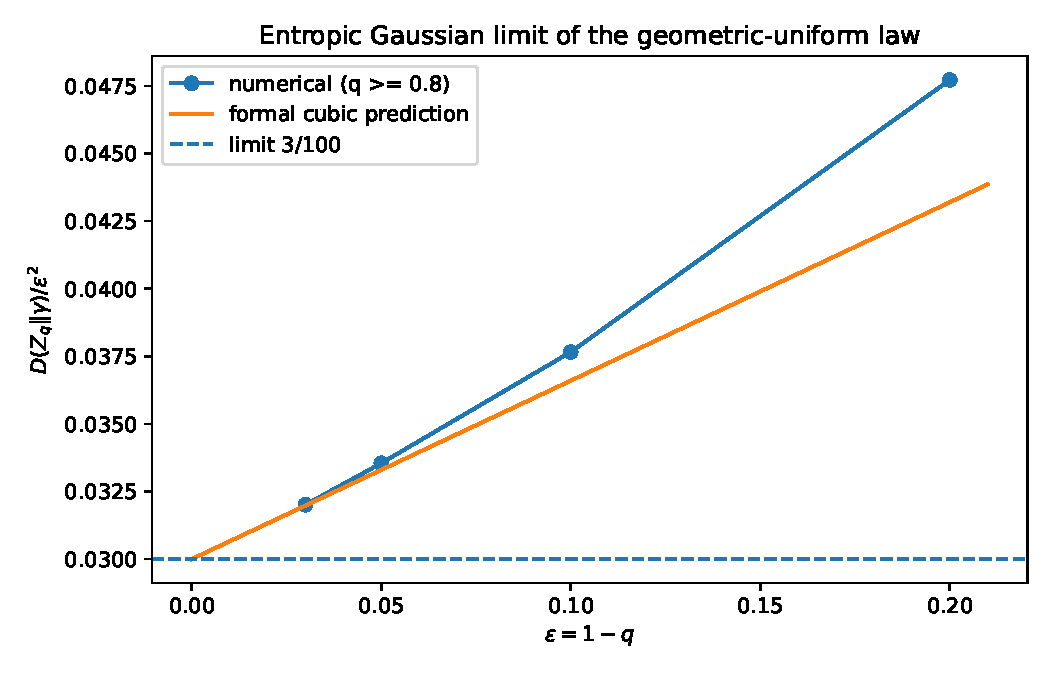
\includegraphics[width=0.86\textwidth]{entropy_deficit.pdf}
\caption{The scaled entropy deficit approaches the predicted limit $3/100$.
The orange line is the formal cubic correction.  Coarser $q$ values remain in the
CSV but are omitted from the asymptotic comparison.}
\label{fig:entropy-deficit}
\end{figure}

\subsection{Dyadic entropy, Fisher information, and finite prefixes}

For the centered Rvachev density the computation gives
\begin{align}
 h(\RvachevUp)&=0.297039912858918,\label{eq:num-hup}\\
 \mathcal J(\RvachevUp)&=11.800710562320129,\label{eq:num-Jup}\\
 V(\RvachevUp)&=0.259694517369981,\label{eq:num-Vup}\\
 \delta_{1/2}&=0.023286331677645\ \text{nats}
 =0.033595075231834\ \text{bits}.
 \label{eq:num-deficit-up}
\end{align}
Thus the predicted finite-prefix coefficient is
\begin{equation}
 \frac{\mathcal J(\RvachevUp)}{18}=0.655595031240007.
 \label{eq:num-prefix-coeff}
\end{equation}

\begin{table}[H]
\centering
\caption{Entropy convergence of the dyadic finite sinc prefixes.}
\label{tab:prefix-entropy}
\small
\begin{tabular}{@{}rrrrr@{}}
\toprule
$m$ & $h(S_m)$ & $h(\RvachevUp)-h(S_m)$ & $4^m[h(\RvachevUp)-h(S_m)]$ & exact MMSE\\
\midrule
1 & 0.000000000 & $2.9703991\!\times10^{-1}$ & 1.1881597 & $2.7777778\!\times10^{-2}$\\
2 & 0.250000000 & $4.7039913\!\times10^{-2}$ & 0.7526386 & $6.9444444\!\times10^{-3}$\\
3 & 0.286463907 & $1.0576006\!\times10^{-2}$ & 0.6768644 & $1.7361111\!\times10^{-3}$\\
4 & 0.294459271 & $2.5806416\!\times10^{-3}$ & 0.6606443 & $4.3402778\!\times10^{-4}$\\
5 & 0.296398474 & $6.4143912\!\times10^{-4}$ & 0.6568337 & $1.0850694\!\times10^{-4}$\\
6 & 0.296879781 & $1.6013200\!\times10^{-4}$ & 0.6559007 & $2.7126736\!\times10^{-5}$\\
7 & 0.296999895 & $4.0018269\!\times10^{-5}$ & 0.6556593 & $6.7816840\!\times10^{-6}$\\
8 & 0.297029910 & $1.0002877\!\times10^{-5}$ & 0.6555485 & $1.6954210\!\times10^{-6}$\\
\bottomrule
\end{tabular}
\end{table}

\begin{figure}[H]
\centering
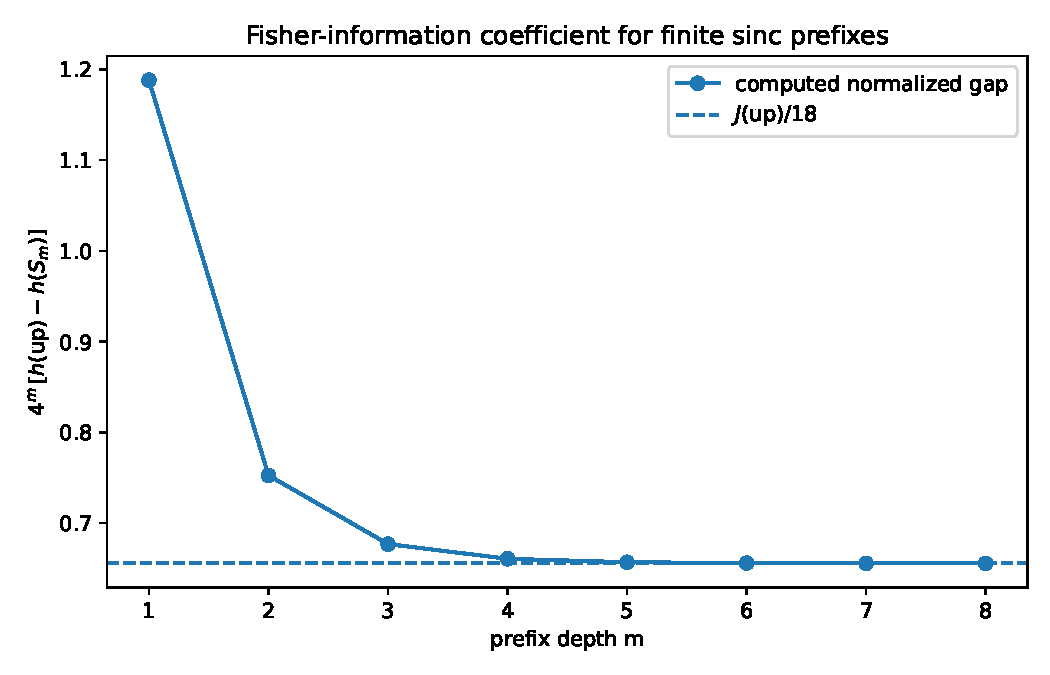
\includegraphics[width=0.86\textwidth]{prefix_entropy_gap.pdf}
\caption{The normalized finite-prefix entropy gap converges rapidly to the
Fisher coefficient $\mathcal J(\RvachevUp)/18$.  Depths beyond eight are retained in the
CSV, but their gaps approach the fixed-grid quadrature resolution.}
\label{fig:prefix-gap}
\end{figure}

\subsection{Information-spectrum convergence}

The limiting variance predicted by \eqref{eq:info-var-limit} is
\begin{equation}
 2V(\RvachevUp)=0.519389034739962.
 \label{eq:num-info-var}
\end{equation}

\begin{table}[H]
\centering
\caption{Monte Carlo information-spectrum check with $180000$ samples.  The KS
column compares the centered information density with a separately simulated
difference of independent Rvachev surprisals.}
\label{tab:info-spectrum}
\small
\begin{tabular}{@{}rrrr@{}}
\toprule
$m$ & centered mean & centered variance & two-sample KS distance\\
\midrule
2 & -0.001960 & 0.472869 & 0.004522\\
4 &  0.001938 & 0.521161 & 0.003367\\
8 & -0.001691 & 0.521082 & 0.004867\\
\bottomrule
\end{tabular}
\end{table}

\begin{figure}[H]
\centering
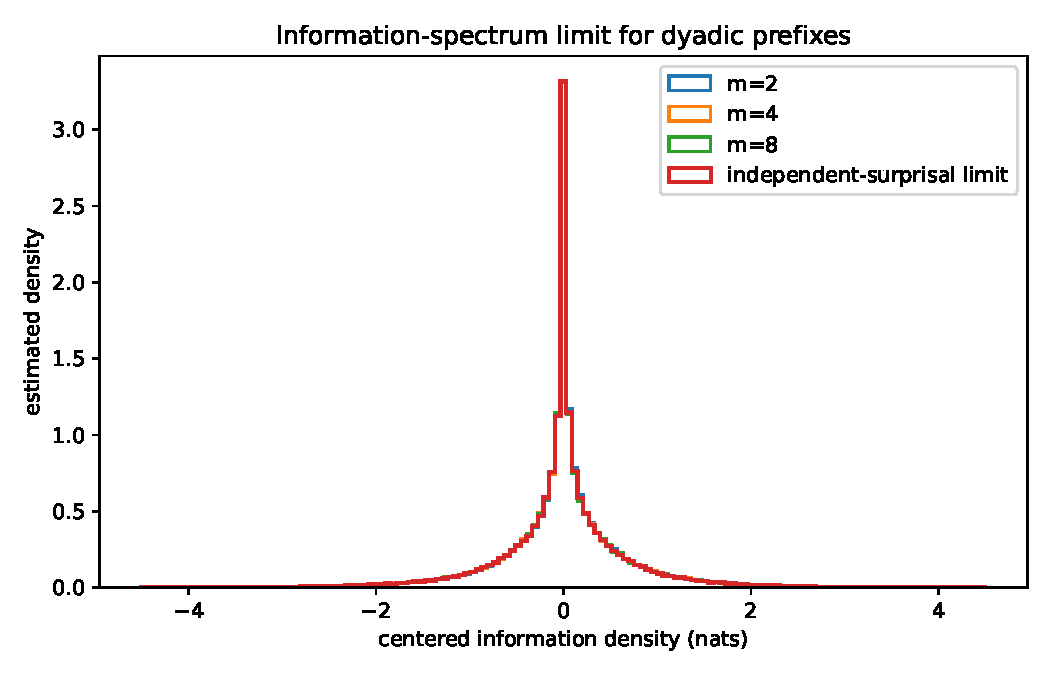
\includegraphics[width=0.86\textwidth]{information_spectrum.pdf}
\caption{Centered information densities at depths $2,4,8$ and the
independent-surprisal limit.  The pronounced central cusp is a genuine
non-Gaussian feature; convergence is not toward a normal information spectrum.}
\label{fig:info-spectrum}
\end{figure}

\subsection{Numerical interpretation}

The experiments support four distinct statements, only one of which is
conjectural:
\begin{enumerate}
\item The exact mutual-information and MMSE laws are symbolic identities; the
      numerics merely provide regression tests.
\item The Fisher coefficient in \eqref{eq:dyadic-fisher-gap} is strongly confirmed
      by the stabilized normalized gaps in \cref{tab:prefix-entropy}.
\item The distributional limit in \cref{thm:surprisal-limit} is confirmed by both
      variance and KS diagnostics.
\item The entropic coefficients in \eqref{eq:formal-entropy-epsilon} agree with
      the $q=0.95$ and $q=0.97$ computations, but the theorem-level uniform
      remainder remains open as stated in \cref{conj:entropic-edgeworth}.
\end{enumerate}

\section{Conjectures and a prioritized frontier program}
\label{sec:frontiers}

\subsection{Full information-spectrum asymptotics}

\begin{conjecture}[Quantitative surprisal convergence]
\label{conj:quantitative-spectrum}
For every compact interval $K\subset(-1,1)$ in the transform variable $t$,
\begin{equation}
 \sup_{t\in K}
 \left|\log\Expectation\EulerE^{t(\imath_m-R_m)}-\Lambda_q(t)\right|
 =O_q(q^m),
 \label{eq:quantitative-spectrum}
\end{equation}
with an all-orders expansion whose coefficients are integrals of score
polynomials in $f_q$.  The same rate should hold in Wasserstein distance for the
centered information density.
\end{conjecture}

A direct route is to write $X_q=\widetilde X_q+q^m(X_q^{(m)}-\widetilde
X_q^{(m)})$ under an independent-copy coupling and Taylor-expand $\log f_q$ away
from the endpoints.  The lower-Lambert endpoint estimates should make the omitted
boundary probability smaller than every power of $q^m$.

\subsection{Optimal coding versus the exact geometric prefix}

\begin{problem}[Exact rate distortion at self-similar points]
\label{prob:exact-RD}
Determine whether $R_{X_q}(D_m)$ admits an expansion
\begin{equation}
 R_{X_q}(D_m)
 =R_m-\delta_q+c_1(q)q^{\alpha_1m}+c_2(q)q^{\alpha_2m}+\cdots,
 \label{eq:RD-expansion}
\end{equation}
with explicit exponents and coefficients.  Decide whether an optimal reproduction
can be chosen from a corrected geometric prefix
$S_{q,m}+q^m\Psi_q(S_{q,m})$.
\end{problem}

The exact posterior makes this unusually concrete: the test channel is known at
all resolutions, and the leading suboptimality is exactly $\delta_q$.  A
high-resolution perturbation of the posterior centroid or companding map may
expose the next coefficient.

\subsection{Periodic Lambert corrections to tail information}

\begin{conjecture}[Phase-resolved endpoint entropy]
\label{conj:tail-phase}
Let $\Psi$ be the period-one lower-Lambert phase from the repository's all-orders
inverse expansion.  There exists an explicit period-one function $\Theta$ such
that
\begin{equation}
 \frac{\mathscr H_F(y)}{y}
 =T-\sqrt{2LT}-\frac L2
 +\frac{\Theta(\rho+\beta)}{\sqrt T}
 +O\!\left(\frac{\log T}{T}\right),
 \label{eq:tail-phase}
\end{equation}
where $\rho=\sqrt{2T/L}$ and $\beta=1/L+1/2$.  The Fourier coefficients of
$\Theta$ should be explicit Gamma--zeta multiples inherited from $\Psi$ and its
derivative.
\end{conjecture}

This is a clean test of how much log-periodicity survives one entropy integration.
The calculation requires no new saddle point: insert the audited all-orders
elasticity into \eqref{eq:tail-entropy-quantile} and apply a derivative-stable
Watson expansion.

\subsection{A Bayesian spectral operator}

Define the normalized posterior pullback
\begin{equation}
 (\mathcal B_mg)(s)
 :=\Expectation\left[g\!\left(\frac{X_q-S_{q,m}}{q^m}\right)
       \middle|S_{q,m}=s\right].
 \label{eq:Bayesian-operator}
\end{equation}
By self-similarity, $\mathcal B_mg$ is the constant $\int g f_q$, so the
normalized residual erases the prefix.  More interesting is the unnormalized
conditional expectation
\begin{equation}
 (\mathcal C_mg)(s)=\Expectation[g(X_q)\mid S_{q,m}=s]
 =\int_{-1}^{1}g(s+q^mz)f_q(z)\Differential z.
 \label{eq:Cm}
\end{equation}

\begin{problem}[$q$-Appell/Legendre singular system]
\label{prob:Bayesian-spectrum}
Diagonalize or triangularize $\mathcal C_m$ simultaneously in the repository's
Appell and Legendre bases.  On polynomials, translation and the exact moments make
$\mathcal C_m$ finite triangular.  Determine whether its finite determinants,
singular values, or exterior powers factor into $q$-Pochhammer products and
Gaussian-binomial coefficients.
\end{problem}

The leading diagonal in an Appell basis is expected to contain $q^{mn}$, while the
translation part should generate a $q$-Weyl algebra closely related to the
existing Koopman calculus.  This would connect the present Bayesian filtration to
the repository's transfer determinants without duplicating the earlier operator
results.

\subsection{Thue--Morse information identities beyond KL}

\begin{problem}[Finite Thue--Morse R\'enyi information]
\label{prob:TM-Renyi}
Evaluate or simplify the order-$\alpha$ R\'enyi mutual information of the dyadic
prefix channel:
\begin{equation}
 I_\alpha(S_m;X)
 =\frac1{\alpha-1}
 \log\iint b_m(s)
 \left(\frac{2^m\RvachevUp(2^m(x-s))}{\RvachevUp(x)}\right)^{\alpha}
 \RvachevUp(x)\Differential x\Differential s.
 \label{eq:TM-Renyi}
\end{equation}
At $\alpha=1$ it collapses to $m\log2$.  At integer orders, substitution of the
finite Thue--Morse spline may produce exact multi-sums controlled by Prouhet
cancellation and the Rvachev moment algebra.
\end{problem}

A particularly tractable case is the collision information $\alpha=2$, where
Parseval and the finite/infinite sinc products may turn the double integral into a
single Fourier integral with valuation-controlled zeros.

\subsection{General masks and higher dimensions}

\begin{conjecture}[Equal-information affine masks]
\label{conj:general-mask}
Let a compactly supported law satisfy an independent affine refinement
\begin{equation}
 X\stackrel d=A X'+\xi,
 \label{eq:matrix-refinement}
\end{equation}
with invertible contraction $A\in\RealNumbers^{d\times d}$ and an absolutely continuous
innovation $\xi$.  For the depth-$m$ innovation prefix $S_m$,
\begin{equation}
 I(X;S_m)=-m\log|\det A|,
 \label{eq:matrix-information}
\end{equation}
provided the relevant differential entropies are finite.  The posterior covariance
is $A^m\Sigma(A^m)^{\mathsf T}$, and the finite-prefix entropy gap has leading term
\begin{equation}
 \frac12\operatorname{tr}
 \left(A^m\Sigma(A^m)^{\mathsf T}\mathcal J_f\right),
 \label{eq:matrix-fisher-gap}
\end{equation}
where $\mathcal J_f$ is the Fisher information matrix.
\end{conjecture}

The mutual-information part follows formally by the same entropy-scaling proof;
the frontier is to formulate minimal hypotheses and connect matrix masks to
multivariate Rvachev atomic functions, box splines, Hadamard masks, and
multivariate Thue--Morse systems.

\subsection{Formalization priorities}

The exact finite layer is well suited to Lean.  A practical order is:
\begin{enumerate}
\item define the geometric prefix and prove the independent tail decomposition;
\item formalize entropy under translation and nonzero scalar multiplication;
\item prove \cref{thm:prefix-information,cor:constant-digit-info,thm:mmse};
\item specialize to $q=1/2$ and connect the finite prefix to the existing
      Thue--Morse spline and Rvachev density APIs;
\item formalize the posterior cumulant and Bell-moment scaling;
\item prove the Fisher bridge \cref{thm:Fisher-bridge} using one-dimensional
      change of variables;
\item postpone \cref{thm:fisher-gap} until a reusable entropy first-variation and
      Fourier-tail library is available;
\item treat the lower-Lambert entropy theorem only after importing the existing
      phase-aware inverse asymptotic interface.
\end{enumerate}
The first five steps are finite or elementary measure-theoretic identities and can
serve as robust regression tests for later analytic formalization.

\section{Conclusion}
\label{sec:conclusion}

The geometric random series behind the Fabius and Rvachev functions carries an
information structure as rigid as its arithmetic and harmonic structures.  A
finite prefix is simultaneously a finite sinc product, a box spline, a
$q$-cumulant truncation, and a sufficient statistic.  The self-similar tail makes
the information filtration exactly linear:
\[
 I(X_q;S_{q,m})=m\log(1/q).
\]
The same identity yields a compact non-Gaussian channel obeying the Gaussian
correlation formula, exact MMSE, and a self-similar rate-distortion curve.
At $q=1/2$, the channel density is an explicit Thue--Morse spline and the
likelihood is a shifted Rvachev atom, closing a finite/infinite sinc loop through
an exact KL integral.

The fluctuation around the linear information law is not Gaussian.  It converges
to a difference of independent surprisals, so varentropy and the complete R\'enyi
curve become natural new invariants of the Fabius--Rvachev law.  The unresolved
tail carries exponentially small information, whose first coefficient is Fisher
information.  This creates a new transform bridge
\[
 \mathcal J(\RvachevUp)
 =\int_0^1\frac{\Differential y}{y(1-y)G'(y)}
\]
and a new asymptotic bridge from finite sinc prefixes to the inverse Fabius
function.  At the flat endpoint, the lower-Lambert quantile scale governs not only
values and derivatives but the entropy contained in a probability tail.

Finally, the exact Bernoulli cumulants organize the near-Gaussian regime.  The
first entropic coefficients $3/100$ and $33/500$ emerge by a finite Hermite
calculation and are accurately reproduced numerically.  Proving the full uniform
entropic expansion, resolving the periodic tail-entropy correction, and
constructing the Bayesian Appell--Legendre spectral system are concrete next
steps.  Together they extend the repository's existing arithmetic, inverse,
$q$-series, sinc, and representation theories in a genuinely different direction:
from exact values and transforms to exact information geometry.

\appendix

\section{Detailed derivations and auxiliary identities}
\label{app:derivations}

\subsection{Entropy-power calculation for the deficit bound}

For completeness, if $a_j=(1-q)q^j$ and $U_j\sim\mathrm{Unif}[-1,1]$, then
\[
 N(a_jU_j)=a_j^2\frac{\EulerE^{2\log2}}{2\pi\EulerE}
 =a_j^2\frac{2}{\pi\EulerE}.
\]
The entropy-power inequality gives
\[
 N(X_q)\ge\frac{2}{\pi\EulerE}\sum_{j\ge0}a_j^2
 =\frac{2(1-q)}{\pi\EulerE(1+q)}.
\]
Thus
\[
 h(X_q)\ge\frac12\log\left(2\pi\EulerE\,
 \frac{2(1-q)}{\pi\EulerE(1+q)}\right)
 =\log2+\frac12\log\frac{1-q}{1+q}.
\]
Subtracting from the matching Gaussian entropy
\[
 \frac12\log\left(2\pi\EulerE\frac{1-q}{3(1+q)}\right)
\]
gives $\delta_q\le\tfrac12\log(\pi\EulerE/6)$.

\subsection{Exact information and correlation in one line}

The prefix variance and tail variance split orthogonally:
\[
 \Variance(S_{q,m})=\sigma_q^2(1-q^{2m}),
 \qquad
 \Variance(q^mX_q^{(m)})=\sigma_q^2q^{2m}.
\]
Therefore
\[
 1-\Corr(X_q,S_{q,m})^2
 =\frac{\Variance(X_q-S_{q,m})}{\Variance(X_q)}=q^{2m},
\]
while entropy scaling gives
\[
 I(X_q;S_{q,m})
 =h(X_q)-h(q^mX_q^{(m)})=-m\log q.
\]
The two identities coincide without any optimization or Gaussian assumption.

\subsection{Formal Hermite entropy algebra}

Let $r=1+u=f_{Z_q}/\gamma$.  Since $\int\gamma u=0$,
\[
 D(f_{Z_q}\|\gamma)
 =\int\gamma(1+u)\log(1+u)
 =\frac12\Expectation_\gamma u^2-\frac16\Expectation_\gamma u^3+O(\Expectation|u|^4).
\]
To cubic order in $\epsilon=1-q$, only
$u_1=(\lambda_4/24)H_4$ contributes after Hermite orthogonality.  Hence
\[
 \frac12\Expectation u_1^2
 =\frac12\frac{\lambda_4^2}{24^2}\,24
 =\frac{\lambda_4^2}{48},
\]
and
\[
 -\frac16\Expectation u_1^3
 =-\frac16\frac{\lambda_4^3}{24^3}\,1728
 =-\frac{\lambda_4^3}{48}.
\]
SymPy verifies
\[
 \lambda_4=-\frac65\epsilon-\frac35\epsilon^2+O(\epsilon^4),
\]
which gives
\[
 \frac{\lambda_4^2-\lambda_4^3}{48}
 =\frac3{100}\epsilon^2+\frac{33}{500}\epsilon^3+O(\epsilon^4).
\]

\section{Corpus-relative nonduplication notes}
\label{app:audit}

The audit compared the present claims with the following major source families in
the recursive tree:
\begin{longtable}{@{}p{0.30\textwidth}p{0.62\textwidth}@{}}
\toprule
Source family & Material treated as existing input \\
\midrule
\endfirsthead
\toprule
Source family & Material treated as existing input \\
\midrule
\endhead
Primary Fabius/Rvachev exposition and glossary & definitions, functional equations, exact arithmetic, probability, Fourier product, moments, corrected asymptotics \\
Lean walkthrough and formalization modules & exact dyadic recurrences, positivity, flatness, logarithmic delay equations, formalized asymptotic interfaces \\
Inverse-and-sampling drafts & inverse derivatives, Lambert $W$, all-orders periodic phase, quantile transforms, sampling and interpolation \\
Exponents and $q$-series drafts & $q$-Pochhammer, Gaussian binomial, geometric comb interpolation, inverse $q$-analogs, parameter asymptotics \\
Integral/fractional-calculus drafts & Mellin, Stieltjes, Cauchy, fractional, primitive, and global quantile-entropy identities \\
Representation drafts & Legendre/Jacobi/Chebyshev/Lagrange expansions, finite synthesis, multiresolution, sampling, Fredholm and Brownian representations \\
Atomic functions beyond dyadic & general-base convolutions, Cantor/nonanalytic sets, derivative energies, R\'enyi entropy, complex dimensions \\
Stein--Koopman report & Appell eigenmodes, $q$-Weyl calculus, transfer determinants, Poisson equations, martingales, Stein kernels \\
Recent frontier reports & negative-$q$ duality, nonanalyticity of iterates, arithmetic-comb algorithms, additional endpoint and transform identities \\
\bottomrule
\end{longtable}

No exact treatment of the geometric-prefix mutual information, posterior MMSE,
information density, varentropy limit, rate-distortion prefix curve, finite-sinc
entropy correction, or Fisher bridge \eqref{eq:Fisher-G} was located.  Existing
entropy statements concern the full quantile integral or different derivative-
energy measures.  The standalone file \path{CORPUS_AUDIT.md} records the search
terms and contribution boundary in a compact form.

\section{Reproducibility manifest}
\label{app:reproducibility}

The ZIP archive contains:
\begin{longtable}{@{}p{0.42\textwidth}p{0.50\textwidth}@{}}
\toprule
Path & Purpose \\
\midrule
\endfirsthead
\toprule
Path & Purpose \\
\midrule
\endhead
\path{fabius_information_frontier.tex} & complete LaTeX report \\
\path{fabius_information_frontier.pdf} & compiled PDF \\
\path{experiments.py} & commented deterministic and Monte Carlo experiment driver \\
\path{requirements.txt} & Python dependency list \\
\path{README.md} & reproduction instructions and file map \\
\path{CORPUS_AUDIT.md} & nonduplication audit summary \\
\path{data/q_entropy_table.csv} & $q$-dependent entropy, Fisher information, and varentropy \\
\path{data/dyadic_prefix_entropy.csv} & finite-prefix entropy and Fisher coefficient \\
\path{data/information_spectrum_summary.csv} & Monte Carlo information-spectrum diagnostics \\
\path{data/thue_morse_signs.csv} & exact finite Thue--Morse signs through depth eight \\
\path{data/symbolic_edgeworth.txt} & exact symbolic cumulant/Hermite check \\
\path{figures/*.pdf, figures/*.png} & vector and raster numerical figures \\
\path{numerical_summary.txt} & human-readable numerical constants \\
\path{SHA256SUMS} & integrity hashes for the archive contents \\
\bottomrule
\end{longtable}

The script requires only NumPy, SymPy, and Matplotlib.  No network access is
required.  The exact theorems do not depend on the numerical experiments.

\begin{thebibliography}{99}

\bibitem{JessenWintner1935}
B.~Jessen and A.~Wintner,
\newblock Distribution functions and the Riemann zeta function,
\newblock \emph{Transactions of the American Mathematical Society} \textbf{38}
(1935), 48--88.

\bibitem{Fabius1966}
J.~Fabius,
\newblock A probabilistic example of a nowhere analytic $C^\infty$-function,
\newblock \emph{Zeitschrift f\"ur Wahrscheinlichkeitstheorie und Verwandte
Gebiete} \textbf{5} (1966), 173--174.

\bibitem{Rvachev1990}
V.~A.~Rvachev,
\newblock Compactly supported solutions of functional-differential equations and
their applications,
\newblock \emph{Russian Mathematical Surveys} \textbf{45} (1990), no.~1,
87--120.

\bibitem{Arias1982}
J.~Arias de Reyna,
\newblock An infinitely differentiable function with compact support: definition
and properties,
\newblock English translation of the 1982 article, arXiv:1702.05442.

\bibitem{Arias2018}
J.~Arias de Reyna,
\newblock Arithmetic of the Fabius function,
\newblock \emph{INTEGERS} \textbf{18} (2018), Article A51;
arXiv:1702.06487.

\bibitem{Haugland2016}
J.~K.~Haugland,
\newblock Evaluating the Fabius function,
\newblock arXiv:1609.07999.

\bibitem{AlloucheShallit2003}
J.-P.~Allouche and J.~Shallit,
\newblock \emph{Automatic Sequences: Theory, Applications, Generalizations},
\newblock Cambridge University Press, 2003.

\bibitem{GasperRahman2004}
G.~Gasper and M.~Rahman,
\newblock \emph{Basic Hypergeometric Series}, 2nd ed.,
\newblock Cambridge University Press, 2004.

\bibitem{Shannon1948}
C.~E.~Shannon,
\newblock A mathematical theory of communication,
\newblock \emph{Bell System Technical Journal} \textbf{27} (1948), 379--423,
623--656.

\bibitem{CoverThomas2006}
T.~M.~Cover and J.~A.~Thomas,
\newblock \emph{Elements of Information Theory}, 2nd ed.,
\newblock Wiley, 2006.

\bibitem{DemboCoverThomas1991}
A.~Dembo, T.~M.~Cover, and J.~A.~Thomas,
\newblock Information theoretic inequalities,
\newblock \emph{IEEE Transactions on Information Theory} \textbf{37} (1991),
1501--1518.

\bibitem{Stam1959}
A.~J.~Stam,
\newblock Some inequalities satisfied by the quantities of information of Fisher
and Shannon,
\newblock \emph{Information and Control} \textbf{2} (1959), 101--112.

\bibitem{Barron1986}
A.~R.~Barron,
\newblock Entropy and the central limit theorem,
\newblock \emph{Annals of Probability} \textbf{14} (1986), 336--342.

\bibitem{BobkovChistyakovGotze2013}
S.~G.~Bobkov, G.~P.~Chistyakov, and F.~G\"otze,
\newblock Rate of convergence and Edgeworth-type expansion in the entropic
central limit theorem,
\newblock \emph{Annals of Probability} \textbf{41} (2013), no.~4, 2479--2512.

\bibitem{Johnson2004}
O.~Johnson,
\newblock \emph{Information Theory and the Central Limit Theorem},
\newblock Imperial College Press, 2004.

\bibitem{Corless1996}
R.~M.~Corless, G.~H.~Gonnet, D.~E.~G.~Hare, D.~J.~Jeffrey, and D.~E.~Knuth,
\newblock On the Lambert $W$ function,
\newblock \emph{Advances in Computational Mathematics} \textbf{5} (1996),
329--359.

\bibitem{Repo2026}
V.~Reshetnikov,
\newblock \emph{ProveIt: FabiusFunction documentation and research-frontier
corpus},
\newblock recursive LaTeX tree under
\path{Analysis/FabiusFunction/docs}, GitHub repository, accessed 30 August 2026,
\url{https://github.com/VladimirReshetnikov/ProveIt}.

\end{thebibliography}

\end{document}
